\documentclass{article}
\usepackage[utf8]{inputenc}
\usepackage{geometry}
 \geometry{
 a4paper,
 total={170mm,257mm},
 left=20mm,
 top=20mm,
 }
 \usepackage{graphicx}
 \usepackage{amsmath}
 \usepackage{titling}

\title{{\em Einschwingvorgänge} or How to turn on an oscillation}
\author{Manuel Eguia}
\date{October 2024}

\usepackage{fancyhdr}
\fancypagestyle{plain}{%  the preset of fancyhdr 
    \fancyhf{} % clear all header and footer fields
    \fancyfoot[R]{\thedate}
    \fancyfoot[L]{\thepage}
    \fancyhead[L]{Turning on Oscillations}
    \fancyhead[R]{\theauthor}
}
\makeatletter
\def\@maketitle{%
  \newpage
  \null
  \vskip 1em%
  \begin{center}%
  \let \footnote \thanks
    {\LARGE \@title \par}%
    \vskip 1em%
    %{\large \@date}%
  \end{center}%
  \par
  \vskip 1em}
\makeatother

\usepackage{lipsum}  
\usepackage{cmbright}
\usepackage{listings}

\begin{document}

\maketitle

\section{One dimensional oscillations on the circle}
We are interested in oscillations as a sound source. So we are interested in some magnitude that continuously changes in time, but remains bounded. The magnitude does not necessarily have to be periodic, but it must be continuous because eventually it will be transformed into a continuous sound.

Further, we will consider this quantity to arise from a deterministic system -- the immediate future state of the system is determined by a rule that depends only on the present state. The state of the system is defined by one or more variables which evolve over time, and it is from these variables that we derive the magnitude to be converted into sound. Because we assume continuous evolution, defining the concept of `immediate future' requires careful consideration.



\subsection{The simplest case (pure tone)}

\begin{figure} [h]
    \centering
    \resizebox*{17cm}{!}{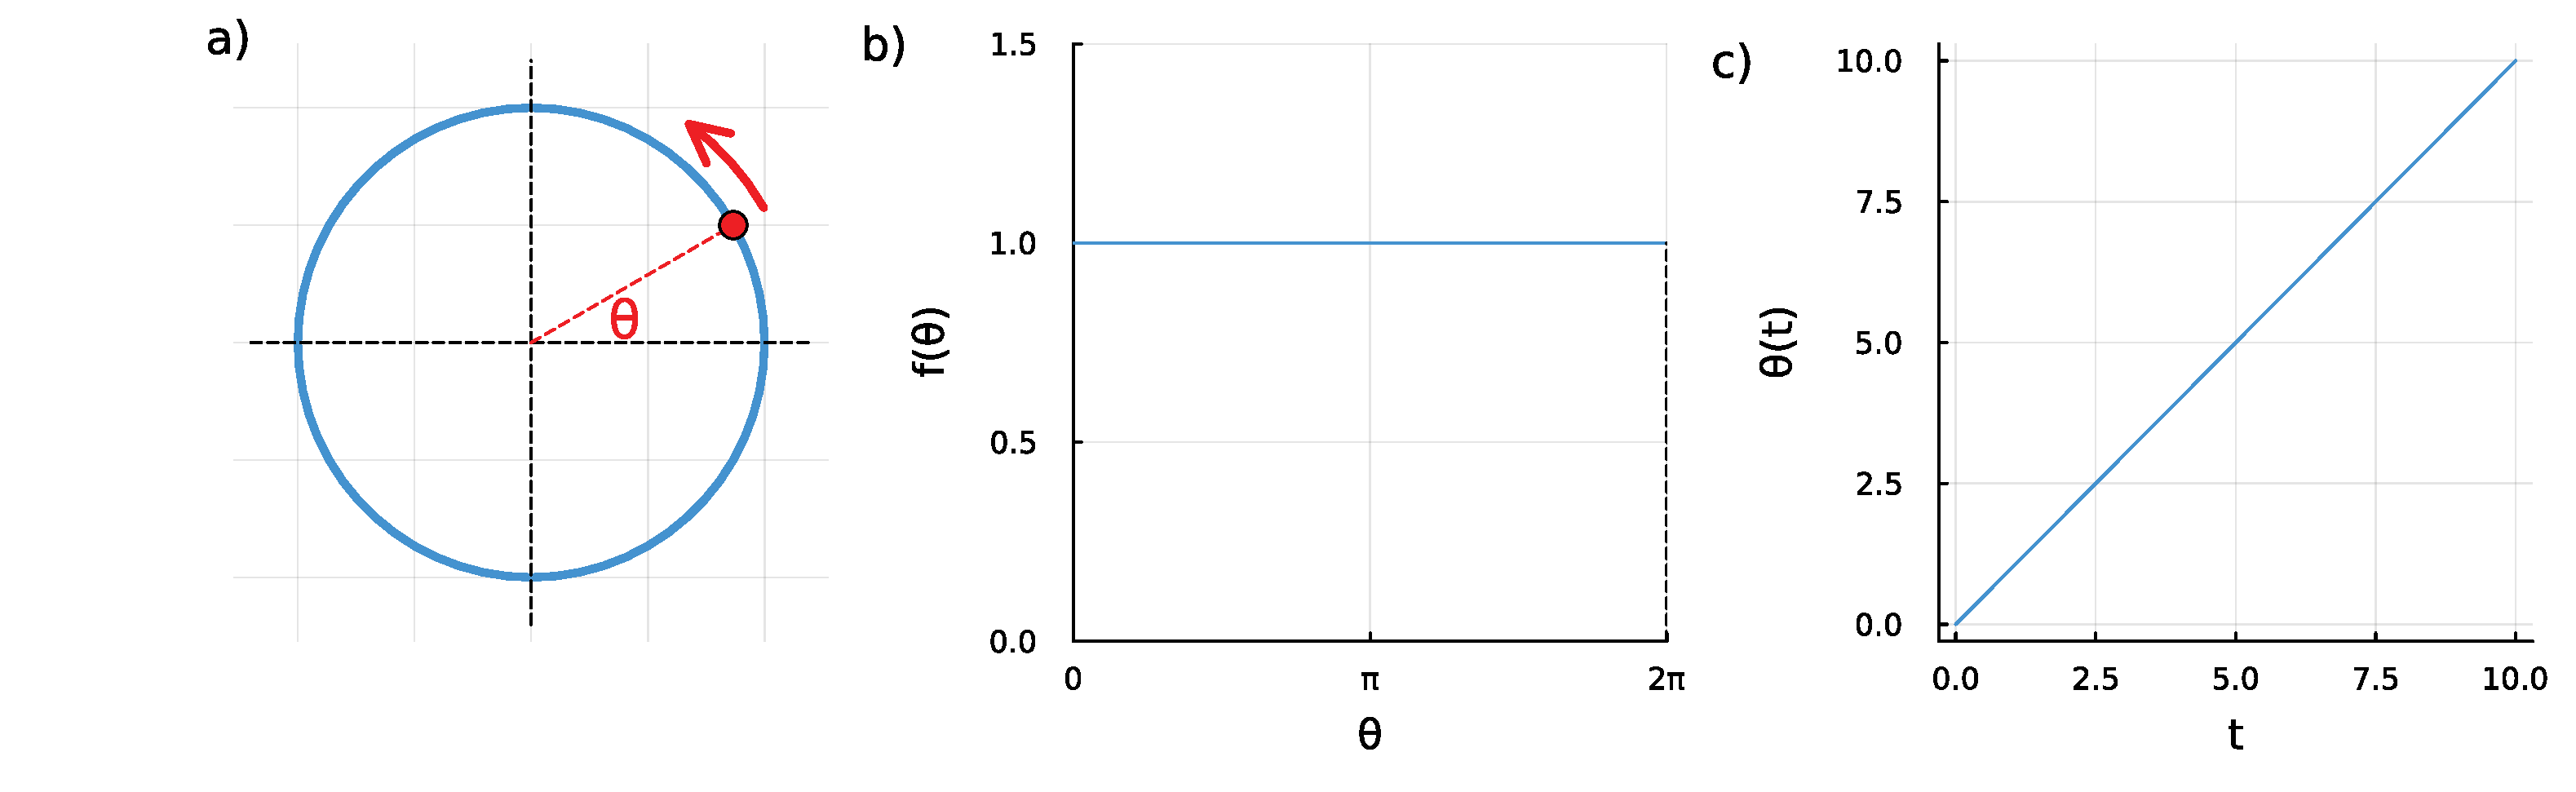
\includegraphics{figure1.eps}}
    \caption{Simplest oscillator given by Equation (1): a) phase space, b) time derivative, and c) time evolution of the variable} 
    \label{fig_pure}
\end{figure}

Let's see an example, perhaps the simplest posible for an oscillator, to understand how this rule must be given. 
Let us consider a system with a state specified by a single angular variable $\theta$. 
We can represent this state as a point on a circle, where its magnitude is the angle on the circle as shown in Figure 1.a.

The representation of a system where each state is given by a single point in the space is known as the {\em phase space} of the system. In this case the phase space is one-dimensional but there can be phase spaces of various dimensions and with different topologies (for example a one-dimensional space corresponding to the straight line is topologically different from the circle).
This state of the system $\theta$ is going to vary in time following some deterministic rule. The magnitude that we will convert into sound will be the horizontal position $\cos(\theta)$.

It should not be surprising that at this point the simplest thing that could be proposed as an oscillation is to postulate that the variable of the system grows linearly with time $\theta(t)=\omega t$ as shown in figure 1.c.  Therefore we have at the output a pure tone, where the variable $\theta$ represents the phase of this oscillator and $\omega/(2\pi)$ its frequency.

\lstset{
basicstyle=\footnotesize 
}
\begin{lstlisting}
(
Ndef(\x, {
	var time = Sweep.ar;   // a constantly rising signal
	var omega = 200 * 2pi; // a frequency of 200 in a circle
	var theta = time * omega; // scaling the time by angular velocity
	cos(theta) * 0.1;      // horizontal component scaled in amplitude by 0.1
}).play // play out through the speakers
)
\end{lstlisting}


However, notice that in that case we are not giving the rule of evolution of the state of the system but the result of that rule, its solution. 
This approach is not general and flexible enough. 
For example, for some rules, it is not possible to calculate the final result. 
Also, the final result depends on the initial state of the system (which will be called {\em initial condition} in the following). Their rules will allow us more general ways of classifying systems than their solutions.

As noted, the evolution rule must describe the immediate future state of the system. 
For a continuous system like this, the rule is provided by the rate of change in time of our variable $\theta$, which, in this case, corresponds to the slope of the line in Figure 1.c. 
Here, the slope is constant at $\omega=1$, meaning the system evolves at a steady angular rate, independent of its initial condition (or initial phase). Figure 1.b displays this rate of change, which as we anticipated is always constant. 
It should also come as no surprise that we call the magnitude represented in this graph the angular frequency (or velocity\footnote{The distinction between angular frequency and velocity is subtle and does not apply to the one dimensional case that we are presenting. In general terms the velocity is a vector while the frequency is a scalar magnitude}) of our oscillator.

Let us then for the moment write the evolution rule as: 

\[
\text{[time-varying rate of]} \quad \theta = \omega
\]

The graphical representation of this rule is given by the graph in Figure 1.b. This means that the rate of change of $\theta$ is uniform, independent of the state of the system. 

Formulating the rule in terms of time-varying rates allows for generalization to scenarios where rates are non-uniform or state-dependent.

\subsubsection{The rule as a differential equation}

We are now ready to give the rule formally using the mathematical concept of {\em derivative}. 
What we wrote earlier as `the time-varying rate of the variable $\theta$' is in fact the definition of the derivative of the variable $\theta$ with respect to time, which we will denote with a dot above the variable. 

Our rule is then finally written as: 
\begin{equation}
\dot\theta = \omega    
\end{equation}

This is what is known as a \emph{differential equation} and is the rule that gives the evolution of deterministic systems with continuous variables. 
In general a differential equation for this variable will be written as follows:

\begin{equation}
\dot\theta = f(\theta)    
\end{equation}

where the derivative with respect to time appears always on the left, and where in general a function $f$ of the state of the system given by our single variable appears on the right.
Note that in the rule given by $f(\theta)$ there is no dependence with respect to time, only with respect to the state of the system.
In the particular case of our simple oscillator this function is constant $f=\omega$ and does not depend on $\theta$. 


\subsection{Non-uniform evolution}

\begin{figure}[h]
    \centering
    \resizebox*{17cm}{!}{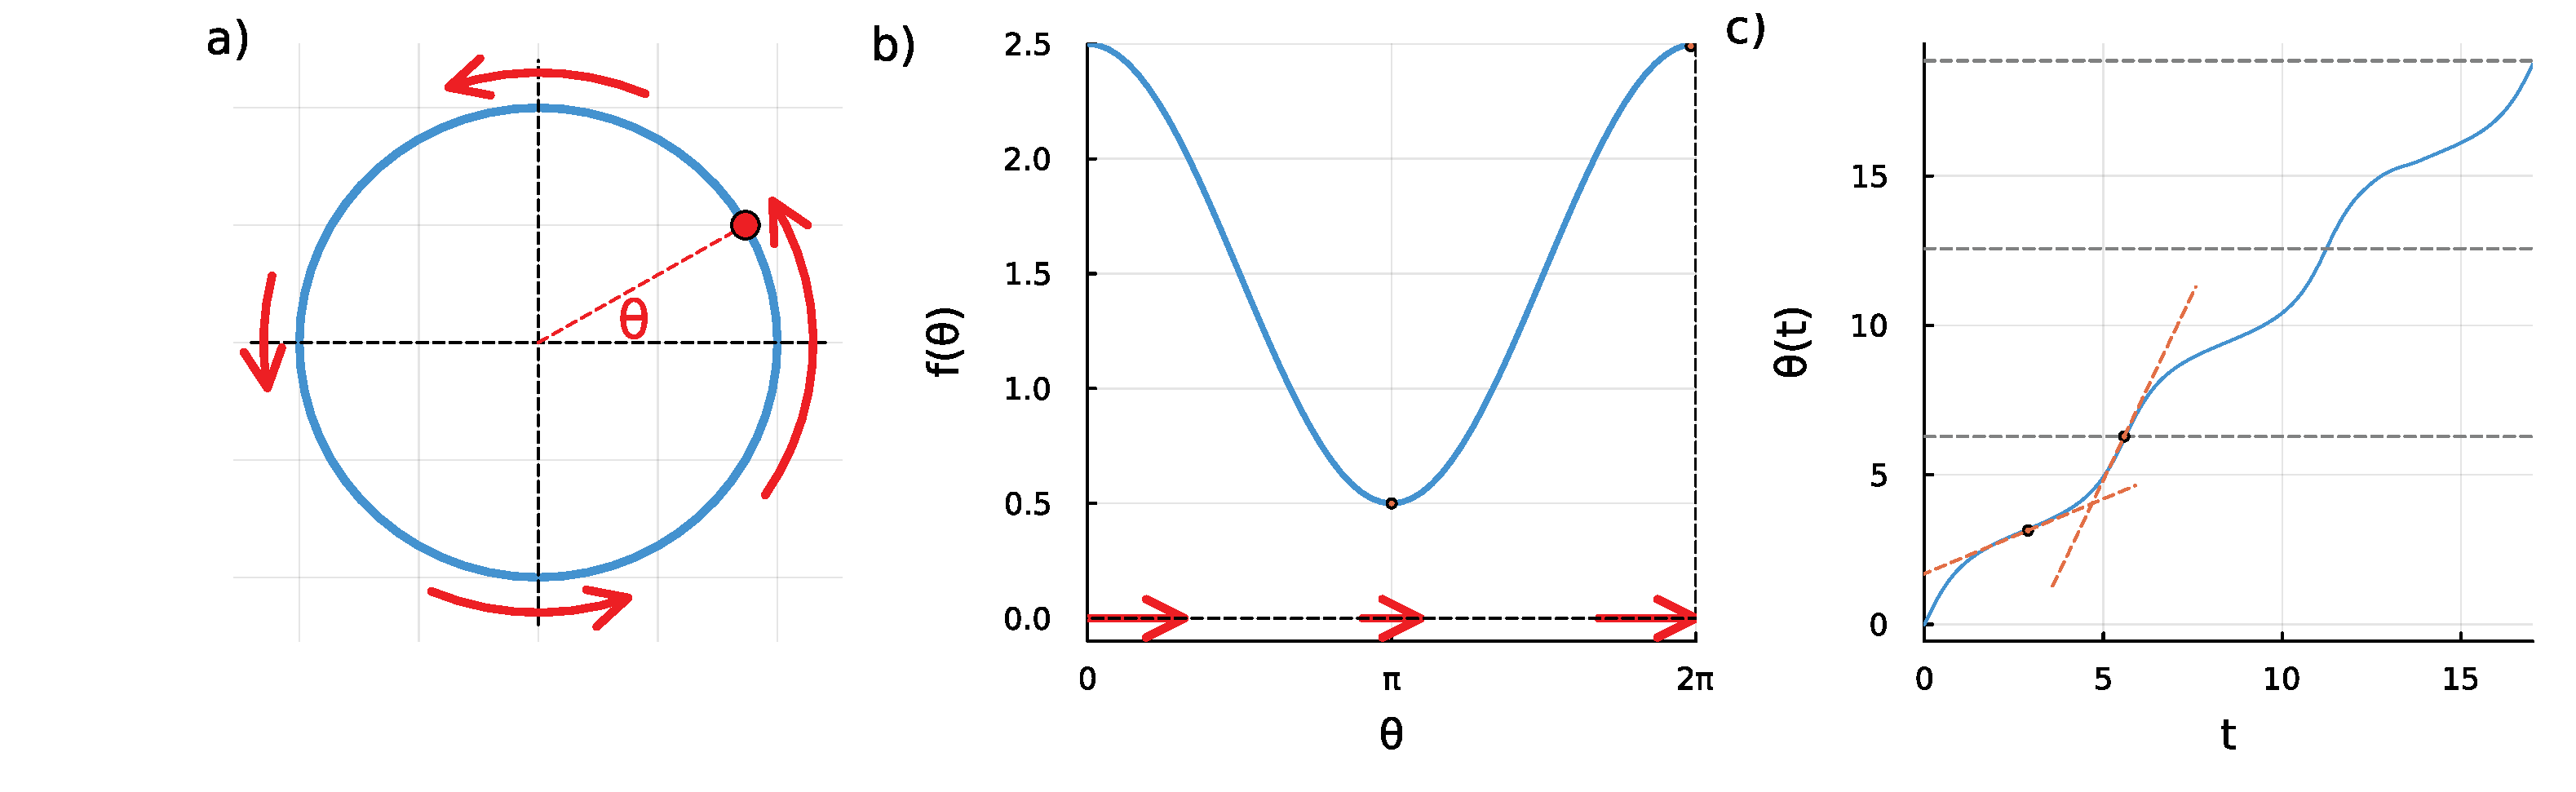
\includegraphics{figure2.eps}}
    \caption{Adler oscillator given by Equation \ref{eq_adler} with $\mu=1.5$: a) phase space, b) time derivative, and c) time evolution of the variable} 
    \label{fig_adler1}
\end{figure}

Our next example will be slightly less obvious. 
From now on, we will avoid providing the solution of the variable~$\theta$ as a function of time like in Figure 1.c. and instead specify the rate-of-change rule for $\theta$ using a graph like the one in Figure 1.b. or, equivalently -- as the differential equation for the time evolution of $\theta$.
It is important to note, because our phase space is a circle, that the states $\theta=0$ and $\theta=2\pi$ represent the same state, so any curve we place in this graph or any function $f(\theta)$ must be periodic in $2\pi$. 
Furthermore, for the moment, we are going to restrict it to be positive for every state, that means that the variable always increases. 

A simple way to create a more interesting scenario than a constant rate of change is to postulate that the angular frequency varies as shown in Figure 2.b. 
Instead of being constant it depends on the angular variable. 
At an angle of 0 (or $2\pi$) has a value of 2.5 while at an angle of $\pi$ it decreases to 0.5.
Before writing our rule as a differential equation, let’s understand what this means in terms of state evolution within the phase space depicted in Figure 2.a. 
The point always moves counterclockwise, but not always at the same speed. On the right side, it moves faster than on the left, and at bottom and top it moves with an intermediate speed, as indicated by the size of the arrows.

Note that we also represent the rate of change on the horizontal axis in the panel b of this Figure using arrows. 
This is exactly as if we were displaying the circle of panel a on the horizontal axis of the graph. 
This qualitative way of representing the rate of change of the state with arrows, which is also known as flow, will be very useful later on.

This could lead to think that the sound result is equivalent to the one obtained by modulating the frequency between 2.5 and 0.5. 
However, it is important to note that unlike traditional FM, this modulation does not occur in a certain way in time, but from a rule that gives the frequency as a function of the phase of the oscillator. 


This distinction is very important and will become evident if we apply the evolution rule and obtain the magnitude transformed to sound, which is shown in Figure 3. 
The waveform obtained is not that of an FM but has a constant frequency and an asymmetric waveform. 
The frequency is constant because once the system returns to the same state after one cycle the behavior will be repeated in exactly the same way. 
And the waveform is asymmetric because the point moves faster in one part of the cycle than in the other.

\begin{figure}[h]
    \centering
    \resizebox*{6cm}{!}{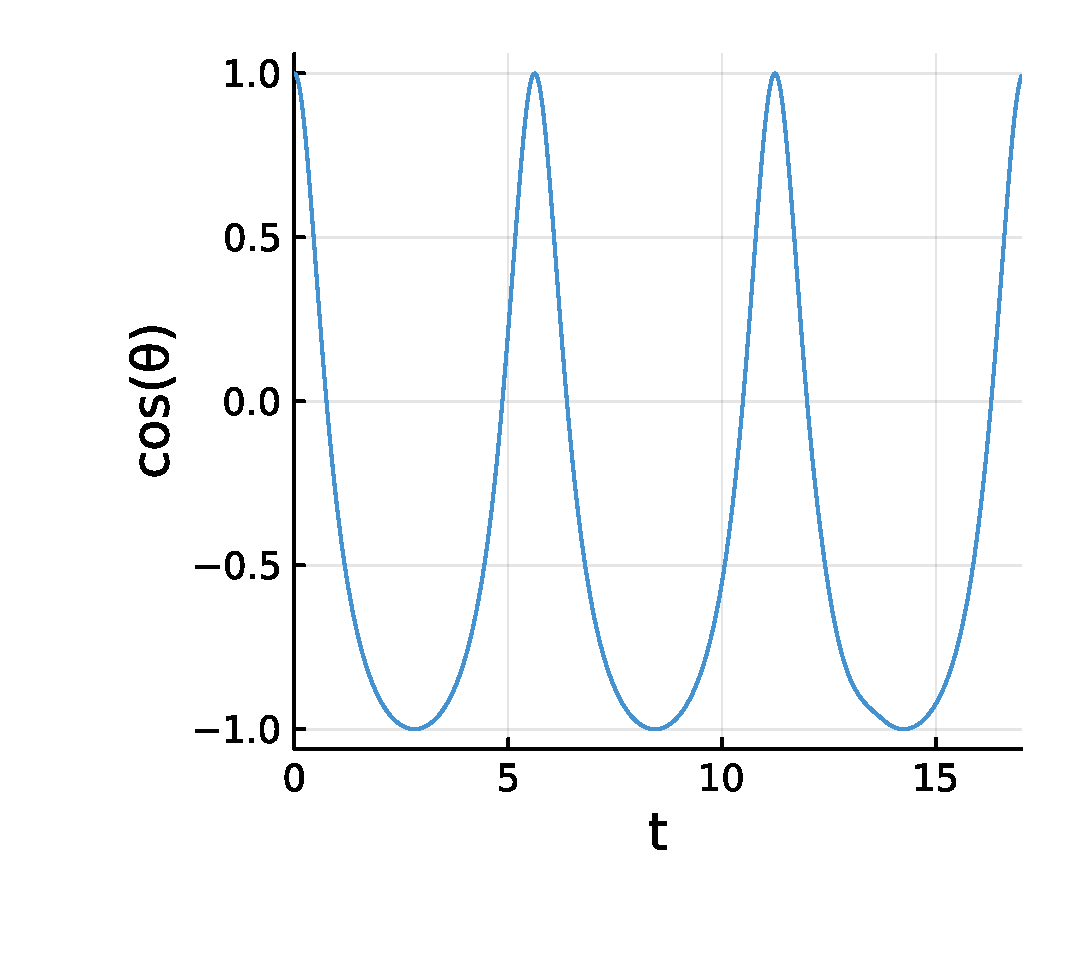
\includegraphics{figure3.eps}}
    \caption{The magnitude to be converted into sound (the cosine of the angle as a function of time) for the Adler's equation (3) with $\mu=1.5$} 
    \label{adler2}
\end{figure}

Let us now write the differential equation governing this system. As before the right hand member $f(\theta)$ indicates the instantaneous angular velocity of the point on the circle as a function of the angle and must be a function of period $2\pi$. 

\begin{equation} \label{eq_adler}
\dot\theta = \mu + \cos(\theta)
\end{equation}

This is known as Adler's equation and is used to model phase locking between oscillators. 
The value $\mu$ represents a {\em parameter} of the system. 
That means, it is a fixed value that once assigned does not change with the evolution of the system. 
For the case we are studying we make $\mu=1.5$ so that $f(x)$ oscillates between 2.5 and 0.5. as shown in Figure 2.b.

This equation cannot be solved in a simple way because unlike an FM we are not specifying the angular frequency as a function of time but instead we are fixing it for each angle value. 
Therefore, as we move on the circle we have to update our angular velocity (the derivative of the angular variable $\theta$) which is equivalent to the slope of the graph of $\theta$ as a function of time shown in Figure 2.c. 
In the graph we also show as an example two instants as orange points where the angle reaches the value $\pi$ and $2\pi$ with their corresponding slopes 0.5 and 2.5. 
If we do this update instant by instant (which is equivalent to integrate numerically our differential equation) we obtain the curve shown in panel c of figure 2: an ever increasing curve, with a slope that varies between 0.5 and 2.5 and that repeats every time it reaches a multiply of $2\pi$ on the vertical axis. 
The cosine of this function in the waveform shown in Figure 3. 
The lower slope parts correspond to the flatter part of the waveform because the point moves slower on the circle and the peaks on the waveform to the faster part on the circle.

At this point we can ask ourselves what would happen with an arbitrary function (as long as it remains periodic and positive). 
We could get very different waveforms but the relationship between $f(\theta)$ and $\cos(\theta)$ is not obvious at all. 
Even more critically, we cannot know in advance the period that the signal obtained will have. 
However, there is something that is intuitive, the greater the value of $f(\theta)$, the faster the point will go along the circle. 
On the other hand, the closer to zero this function gets, the slower the time evolution will become. 

\begin{figure}[h]
    \centering
    \resizebox*{17cm}{!}{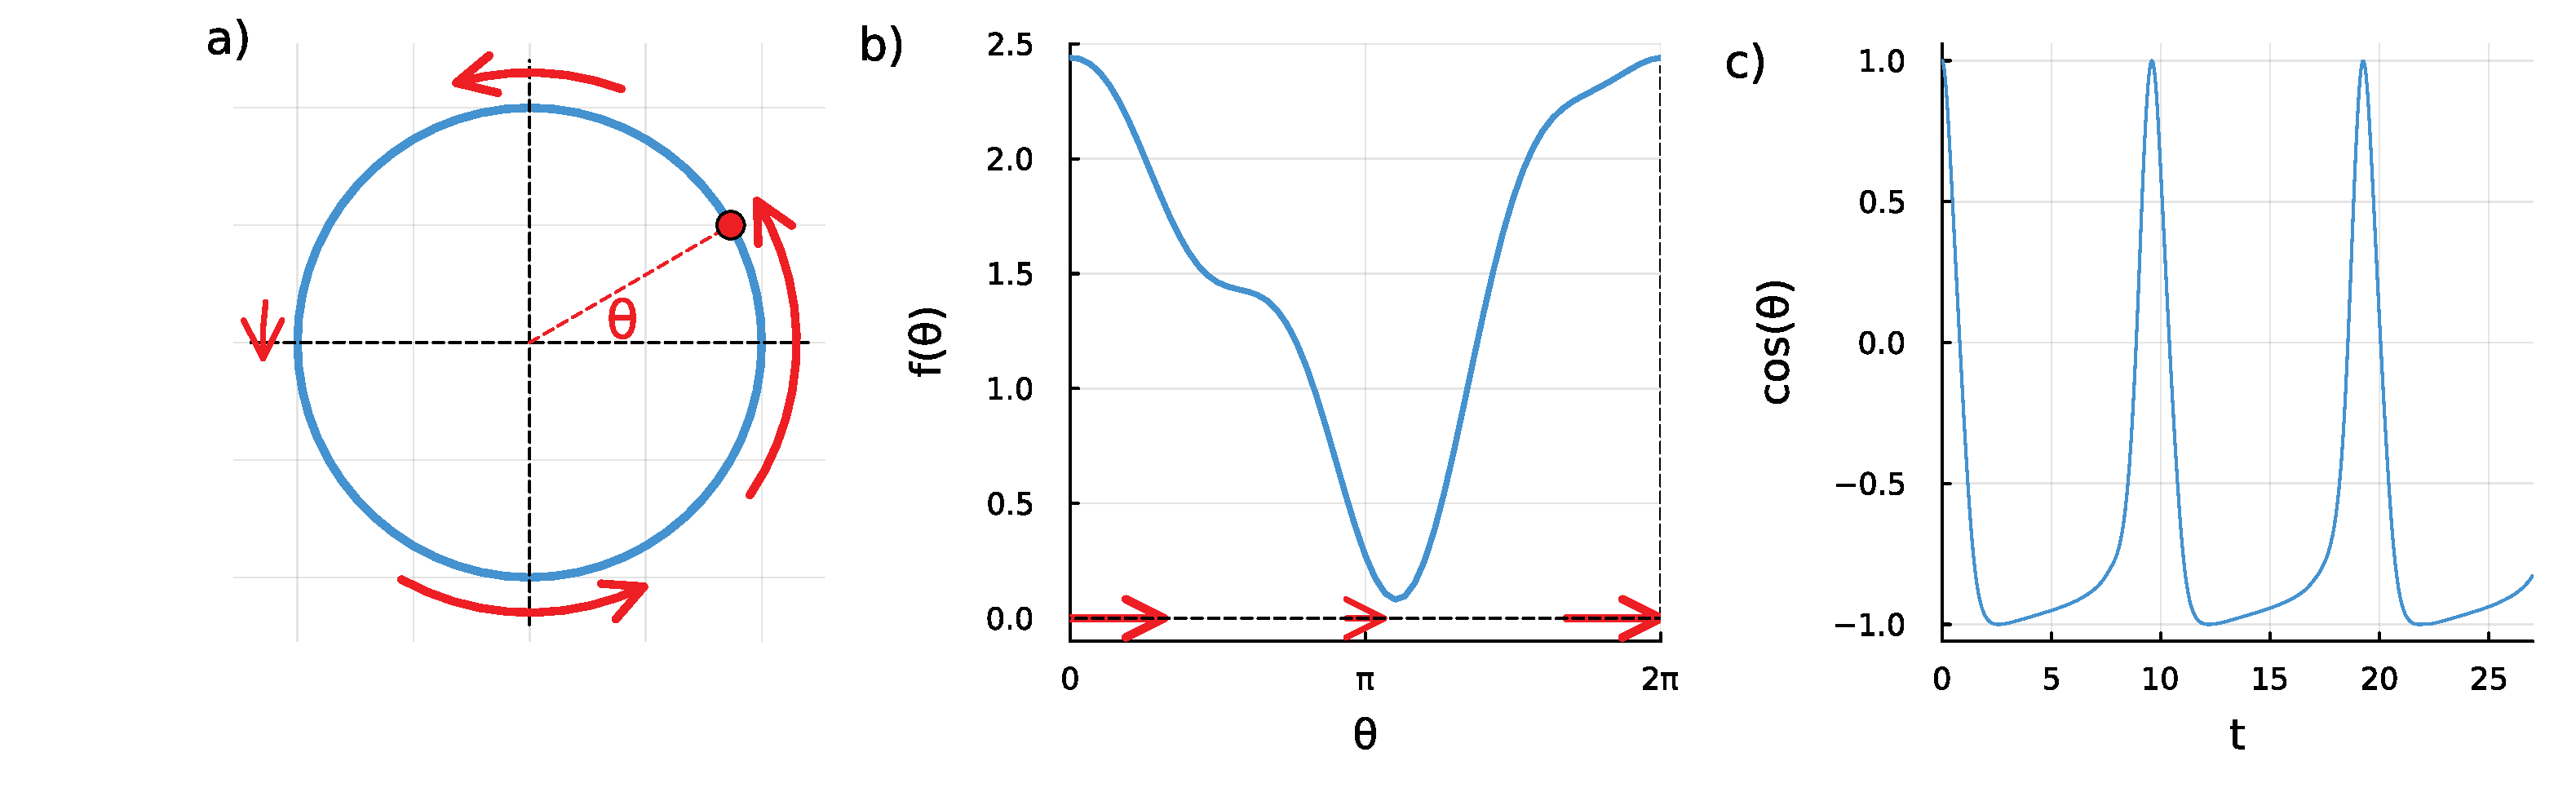
\includegraphics{figure4.eps}}
    \caption{A more general oscillator with an arbitrary periodic positive function $f(\theta)$ displayed in panel b. Panel a and c display the 
    phase space and the time evolution of the cosine of the angle respectively} 
    \label{fig_adler3}
\end{figure}

In Figure 4 we display a more complex function $f(\theta)$ (built with periodic functions but it is not worth to write the differential equation) having a risky approximation to zero for an value of $\theta$ slightly higher than $\pi$ (see panel b of Figure 4). 
In this zone, which corresponds to the left part of the circle in the phase space in Figure 4.a, the motion of the point (or flow) becomes very slow as indicated by the small arrow. 
As expected, this produces a flatter part of the waveform even than in the previous case because the flow slows down much more.




\subsection{The end of an oscillation}



\begin{figure}[h]
    \centering
    \resizebox*{17cm}{!}{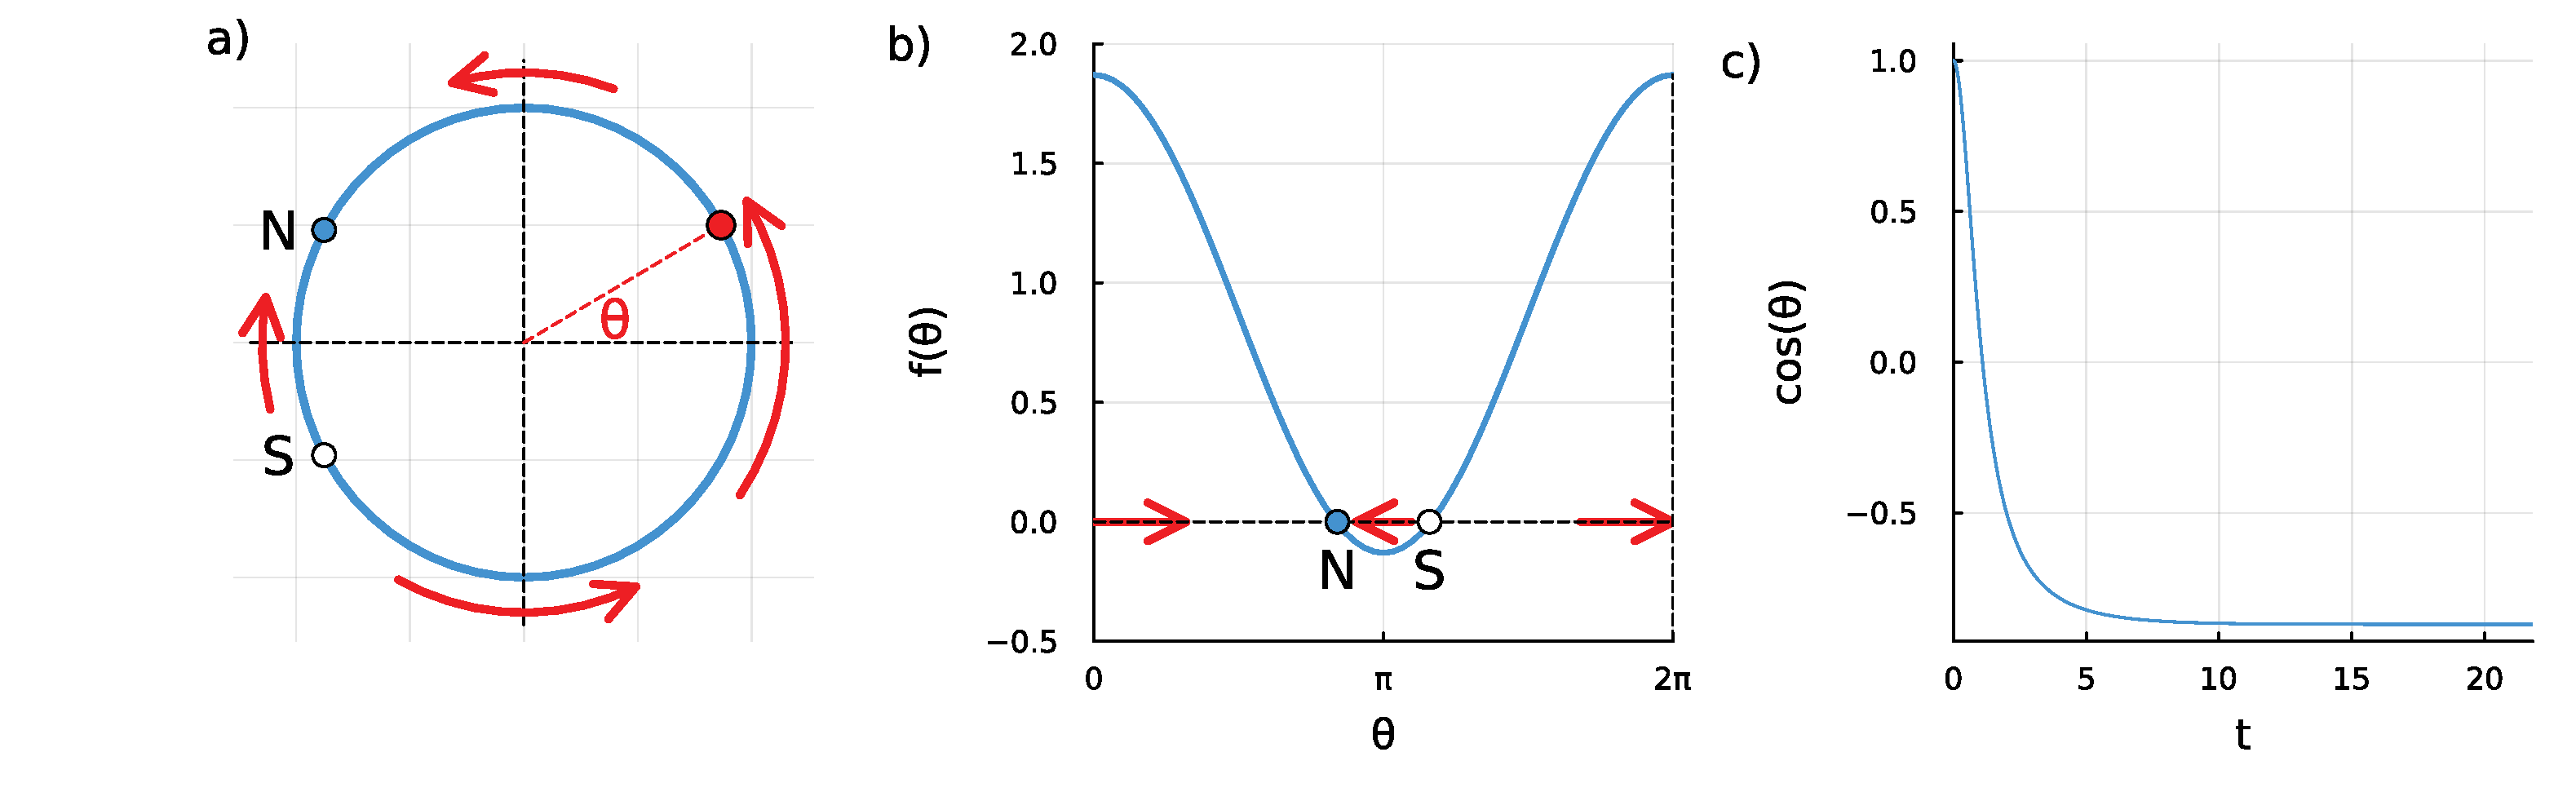
\includegraphics{figure5.eps}}
    \caption{Adler oscillator given by Equation (3) with $\mu=0.9$: a) phase space, b) time derivative, and c) the cosine of the angle as a function of time} 
    \label{fig_adler4}
\end{figure}

The next step then is to ask what happens if the function $f(\theta)$ reaches the value zero or crosses the horizontal axis. That is, if we eliminate the requirement that we had put before that this function must be positive for all $\theta$ values. 

Let us return to the original system of the Adler equation but now with a value $\mu=0.9$. This is shown in Figure 5.b. 

Notice that now $f(\theta)$ varies between 1.9 and -0.1 which means that there is a short interval around $\pi$ in which the function is negative. 
This means that in that interval the rate of change of the variable is negative so the point in phase space should go in the opposite direction as indicated by the arrow in Figure 5. 
In other words, unlike before where the value of the variable was always increasing (with greater or lesser rate) now it decreases and the flow moves in the opposite direction at least in part of the phase space.  

The points where the arrow changes direction are indicated as circles with the letters S and N in panels a and b of the Figure 5 and correspond to what are known as fixed points. These fixed points are exactly the points where the function $f(\theta)$ crosses the horizontal axis since there the rate of change is zero and the value remains constant. 
In other words, if the system starts in that state its derivative is zero and therefore does not vary and remains at that value forever which explains the name fixed point. 

Note that there is an important qualitative difference in what happens in a neighborhood of both fixed points. 
In the neighborhood of the fixed point indicated as N the arrows converge to it therefore it is said to be a stable fixed point or Node.  
While in the other fixed point the arrows diverge from it and it is an unstable fixed point. The S stand for Saddle point and the meaning of this term will make sense when we go to a higher dimensional phase space.

What will happen then in the dynamics of this system? 
Any trajectory that starts at an angle where the function is positive will rotate counterclockwise and will approach the node. 
Technically it will never reach it because the flow will become slower and slower around it (it can be shown mathematically that the function of the variable with respect to time corresponds to an exponential decay towards the value of the variable at the node). 
And no matter where we start from we will always tend to the Node, either from the clockwise direction (if we start whitin the shortest arc between N and S) or from the counterclockwise (if we start from any other point). 
This means that there is no more oscillation and we have a decay to a stable fixed point.
This is displayed in Figure 5.c

Let us review then what happened. 
As long as we had a positive function $f(\theta)$ the variable $\theta$ is always growing, with different rates of change, and we have an oscillatory behavior with a waveform with flatter parts in the slower regions and peaks in the faster regions. 
But as soon as the function crosses zero the oscillation disappears. 
So we have not shown how to turn on an oscillation but how to turn it off. 

And this change goes along with the appearance of two fixed points a node and a saddle where before there was a region of very slow flow. 
Later we will see that this qualitative change corresponds to what is known as a {\em bifurcation} of the dynamical system and in particular this is a Saddle-Node Bifurcation on the Circle. 

In the particular case of the Adler equation this bifurcation occurs for $\mu=1$. 
This is because for $\mu$ values greater than one we have an oscillation and when $\mu$ becomes less than one the oscillation disappears. 
Here we see a relevant meaning of the notion of parameter of a system. 
During the time evolution the parameter is fixed, but knowing the value of the parameter one can know the qualitative behavior of the system, i.e. whether there will be an oscillation or not.

It is interesting that this process can happen the other way around. 
That is, the value of $\mu$ can have a positive value less than one and in that case there is no oscillation. But if for some reason the system changes and $\mu$ exceeds one, an oscillation starts. 
This means that the Saddle Node Bifurcation on the Circle is one of the ways (perhaps the simplest) in which an oscillation can be turned on. 

\subsection{Questionnaire}
\begin{enumerate}
    \item In Figure 1.c the time evolution for a initial state $\theta=0$ is portrayed. How could the ensemble of all possible initial conditions between 0 and $2\pi$ be represented in this graph?
    \item Is it possible to have an evolution in which the point moves clockwise on the circle? How would the graph of $f(\theta)$ in Figure 1 and the differential equation (1) change?
    \item Why it is necessary to take the cosine of the variable $\theta$ in order to have a magnitude that can be converted into sound?
    \item Make a qualitative diagram of how Figure 2 would change if the differential equation had $\cos(2\theta)$ instead of $\cos(\theta)$. Draw a qualitative sketch of the waveform.
    \item What happens to the system given by the Adler's equation when the parameter $\mu$ is exactly equal to 1. Are there fixed points? How does the flux in phase space and the waveform change?
    \item In the text it says that the oscillations disappear for $\mu$ less than 1. Is this strictly true? What happens for negative $\mu$ values?
    \item What happens if the system is at node N and we add a small perturbation in the variable? And how does it change if we add the perturbation when the system is in the saddle S? 
    \item Suppose we are at a value very close to the bifurcation with the value of $\mu$ slightly below 1. This implies that the node and the saddle are very close. What happens if the system is decaying to the node and we add a perturbation? Distinguish whether the perturbation is positive or negative.
\end{enumerate}
\section{Two dimensional self-sustained oscilations}

\subsection{Impossibility of oscillations in one dimension (on the straight line).}

The previous system was defined by the evolution of a single variable, namely that the value of that variable univocally determines the state of the system.
The phase space, which is defined as the space of all possible states where each state corresponds to a single point in that space and vice versa, was therefore one-dimensional. 
However, a peculiarity of the previous phase space is that the state was defined by the angle and was therefore a circle. 
Any angle by adding or subtracting $2\pi$ corresponds to the same state. 
In general a continuous variable that does not have this requirement can be associated to a phase space on a straight line.
In this case our differential equation for the $x$ variable in the straight line:

\begin{equation}
    \dot x = f(x)
    \label{eq_1d}
\end{equation}

will define the evolution through the arbitrary function $f(x)$. 
If we represent this arbitrary function superimposed to the line we can plot with arrows qualitatively where the system will evolve as shown in Figure 6.

\begin{figure}
    \centering
    \resizebox*{6cm}{!}{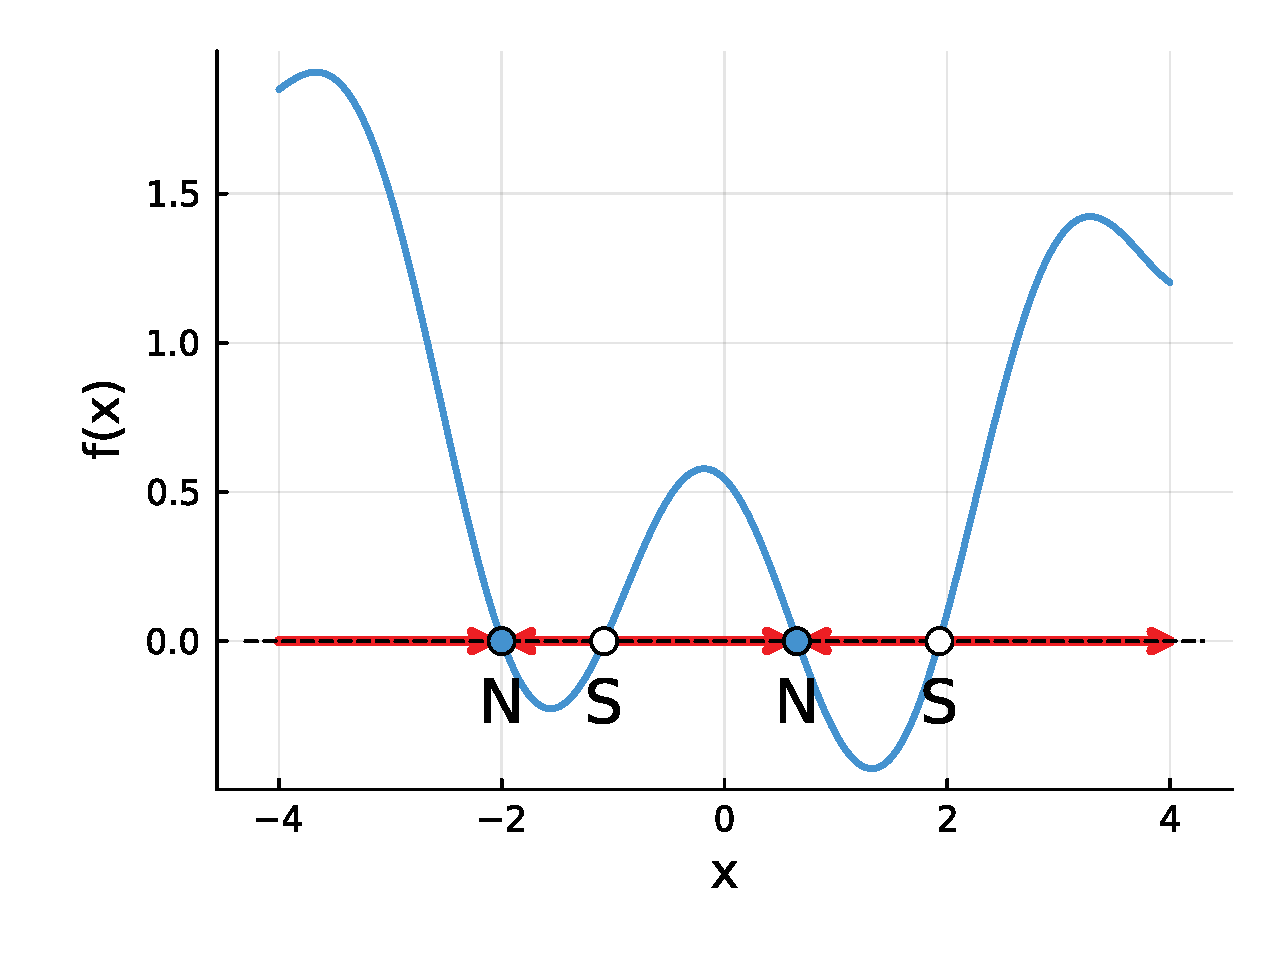
\includegraphics{figure6.eps}}
    \caption{An arbitrary function $f(x)$ for the time evolution of the one-dimensional dynamical system given by equation \ref{eq_1d} and the flow in the phase space given by the red arrows} 
    \label{fig_onedimension}
\end{figure}

In all the intervals where the function is positive the derivative with respect to time is positive and the evolution increases the variable, i.e. the flow is to the right. 
And in turn, in all the intervals where the function is negative the time derivative is negative and the evolution decreases the variable and the flow is to the left.

As in Figure 5 the points where the function crosses the horizontal axis correspond to fixed points and if the arrows converge towards them are stable nodes (N) and if the arrows diverge they are unstable or saddle points (S). 
Note that we can also distinguish S and N points by the slope of the function when it crosses the horizontal axis. 
If the slope is negative the arrows converge (it is an N) and if the slope is positive the arrows diverge (an S point). 
Any initial condition in this system will evolve approaching the nearest node N and will stay in its neighborhood. In other words, it is not possible to have oscillations in any one-dimensional system on the line. 

Another way of looking at it is that no evolution can cross the same point twice going in two different directions, which would be equivalent to having two arrows at the same point. 
Note that this is because precisely the definition of our systems is that their evolution is univocally determined by their present state which corresponds only to one point in the phase space and if that point had two arrows it would have two futures. 
The “trick” that allowed to have oscillations with only one variable in the previous case was to curve the phase space of the straight line to form a circle. 
In that case an always positive evolution corresponds to an oscillation around the circle. 
In other words, the oscillation was possible only because of the particular topology of the phase space. 

\subsection{The simplest physical oscillator (harmonic)}

To have oscillations without any “tricks” with phase space topology we need to go into two dimensions. 
That is, we need at least two continuous variables in a phase space on the plane in order to have oscillations. 

This is a well-known result from physics. 
In order to describe an oscillator we need at least two variables: its position and its velocity, since with only the position we cannot univocally determine its state. 
A mass attached to a spring or a pendulum passes twice through the same position but with two different velocities and that is something constitutive of the oscillation. 
Therefore, if we say that the state of the system is univocally determined by the value of its variables, a physical oscillator needs at least a two-dimensional phase space. 

\begin{figure}
    \centering
    \resizebox*{17cm}{!}{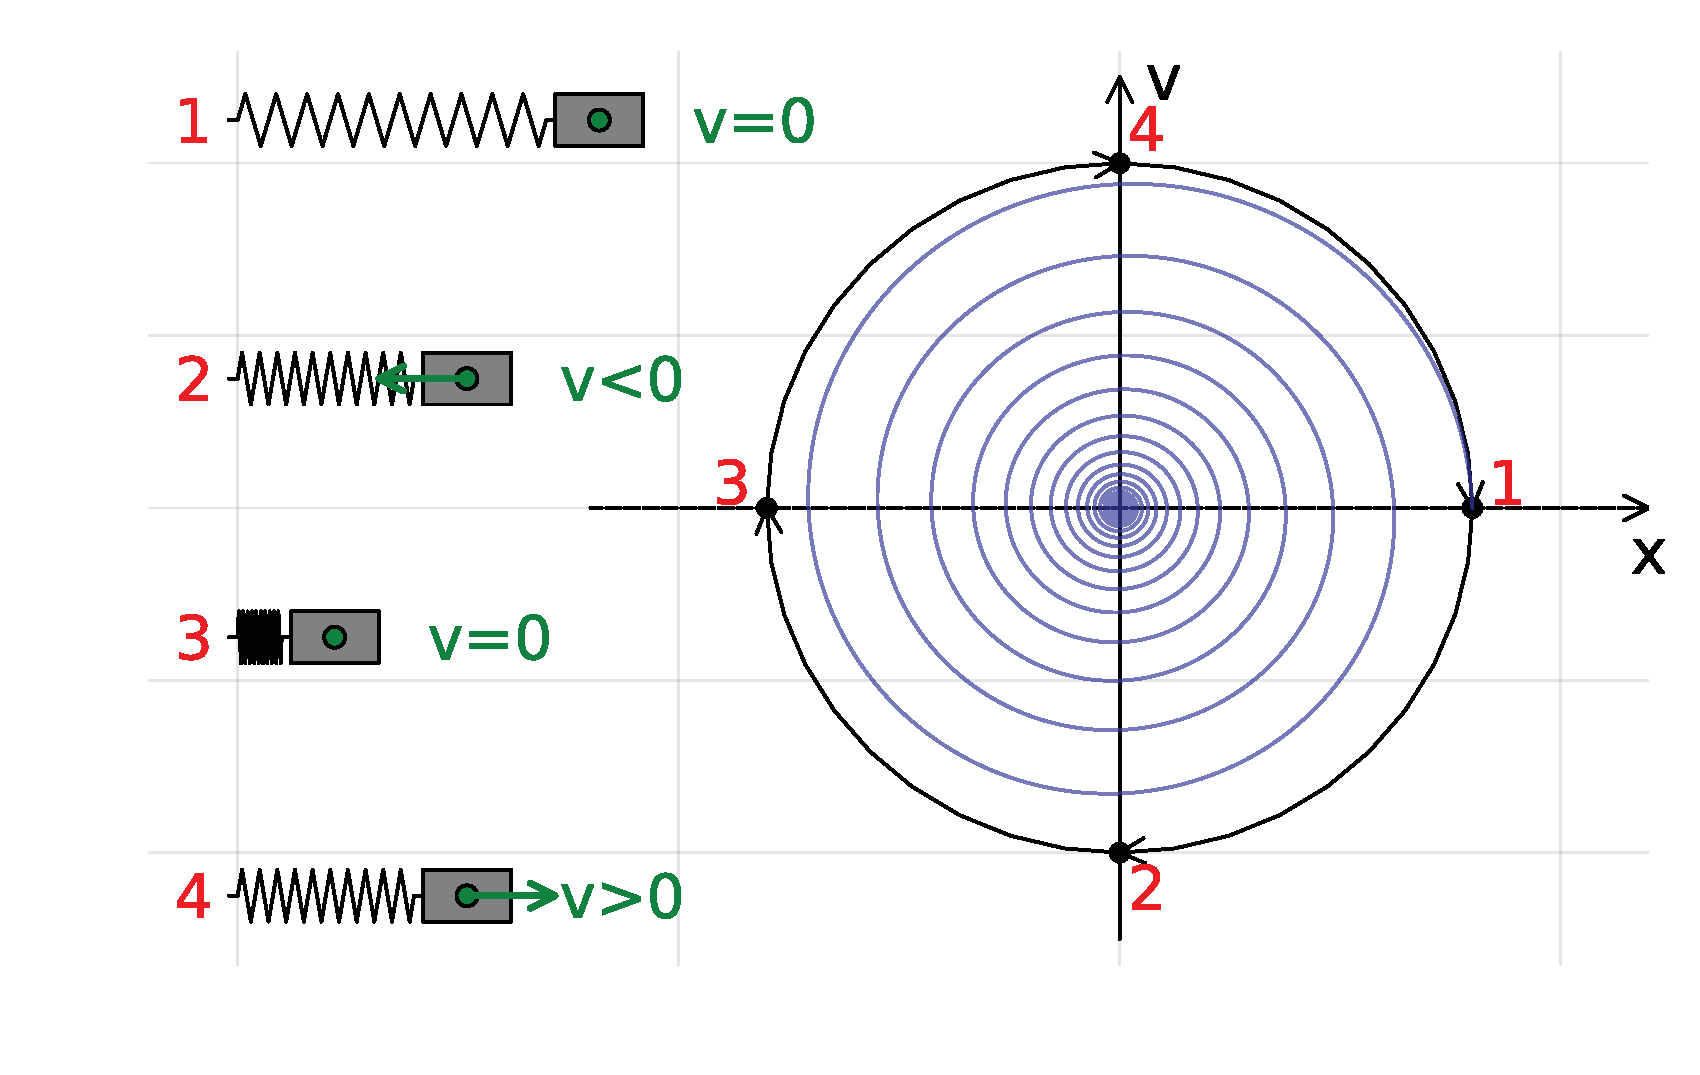
\includegraphics{figure7.eps}}
    \caption{Phase space representation of four states (1-4) of the ideal harmonic oscillator without dissipation (center) portrayed as a spring-mass system in the left, and time evolution of the $x$ variable for the case with dissipation (blue trajectory in the phase space)} 
    \label{fig_harmosc}
\end{figure}

And since we used the mass-spring system as an example we can make those variables the position and velocity of this simple oscillator. 
Figure 7 shows a mass attached to a spring and four stages in its oscillation. 
The position is indicated by the horizontal coordinate ($x$) and the velocity by the green arrow ($v$). In the central panel this state is represented on the phase space ($x,v$).
It is not difficult to see that the evolution of this system results in a cycle in phase space that closes on itself when there is no energy dissipation. 
Starting from the initial position on the right, with the spring stretched and zero velocity (1), the system accelerates leftward due to the spring’s force, passing through the midpoint with maximum negative velocity (2). It then continues until reaching maximum compression on the left, where velocity drops to zero (3). At this point, it begins accelerating rightward, passing through the midpoint again with maximum positive velocity (4), and stretches the spring until it returns to the initial state.

Of course this is an idealized case and in a real situation there are always dissipative forces \footnote{We will use the terms "dissipation" and "damping" interchangeably; however, it's worth noting that the oscillator is damped due to the dissipation of energy. This energy dissipation may be caused by various factors, including (but not limited to) friction.} acting either by internal friction or with the air.
In this case, the system does not return precisely to state 1 but instead reaches a position with slightly less amplitude in elongation each cycle. 
As a result, the system's actual trajectory in phase space forms the blue spiral shown in Figure 7. 
With each cycle, the system experiences reduced elongation on the right, less compression on the left, and a lower velocity as it passes through the midpoint. 
Gradually, this spiral converges toward the center (x=0, v=0), which, as is easy to imagine, represents the rest state.

To write the differential equations that give the evolution of this system we can recur to the laws of Newton, which in this case have a simple expression. 

\begin{subequations} \label{eq_harmosc}
\begin{align}
    \dot{x} & = v \\
    \dot{v} & = -\gamma v -kx 
\end{align}
\end{subequations}

The first equation links the velocity with the derivative of the position in time. 
In fact that is the actual definition of velocity. 
The second equation is Newton's second law of movement which gives the proportionality between the time derivative of the velocity on the left $\dot v$ (i.e. the acceleration) with the sum of the acting forces on the right. 
And these forces are two: on the one hand the elastic force that opposes the displacement linearly with a constant $k$, and a dissipative force that acts a resistance, always opposing the movement with a constant $\gamma$.

The result of the evolution of this system is the spiral shown in figure 7. 
This means that for each initial condition the evolution in the phase space is a spiral approaching the origin where there is a single fixed point which is an attractor node. One example of such evolution is displayed in the right panel of Figure 7. As can be seen, the variable $x$ oscillates around the origin while decaying (exponentially) to the steady state.

As an exercise we can study how the parameters $k$ and $\gamma$ affect the result and if we transform in sound some of the two variables we can study if there is a simple relation between the frequency and the parameter $k$.

\subsection{Turning on the oscillation (Hopf Bifurcation)}

The simple harmonic oscillator, although physically realistic, is not very interesting as a sound generator (except as an approximation to the point excitation of a single oscillation mode). 
We are interested in how we can keep an oscillation on and if possible a system whose final oscillation does not depend on the initial condition. 
This can be achieved by self-sustained oscillations and there are several ways to accomplish this. 

Perhaps the simple way to obtain self-sustained oscillations is to introduce a negative resistance that acts as a positive feedback for small oscillations.
This can be done by replacing the linear damping force $\gamma v$ for some non-linear function that is positive for small values of the velocity $v$ and negative for larger values.
The positive part drives the system by supplying energy when the amplitude of the oscillations are small and the negative part acts as a strong nonlinear damping that prevents the unbounded buildup of energy for larger oscillations. 
In its simplest form we can think of a nonlinear damping in the form of $\gamma v - v ^ 3$.

\begin{subequations} \label{eq_selfosc}
\begin{align}
    \dot{x} & = v \\
    \dot{v} & = \gamma v - v^3 -kx 
\end{align}
\end{subequations}


\begin{figure}
    \centering
    \resizebox*{17cm}{!}{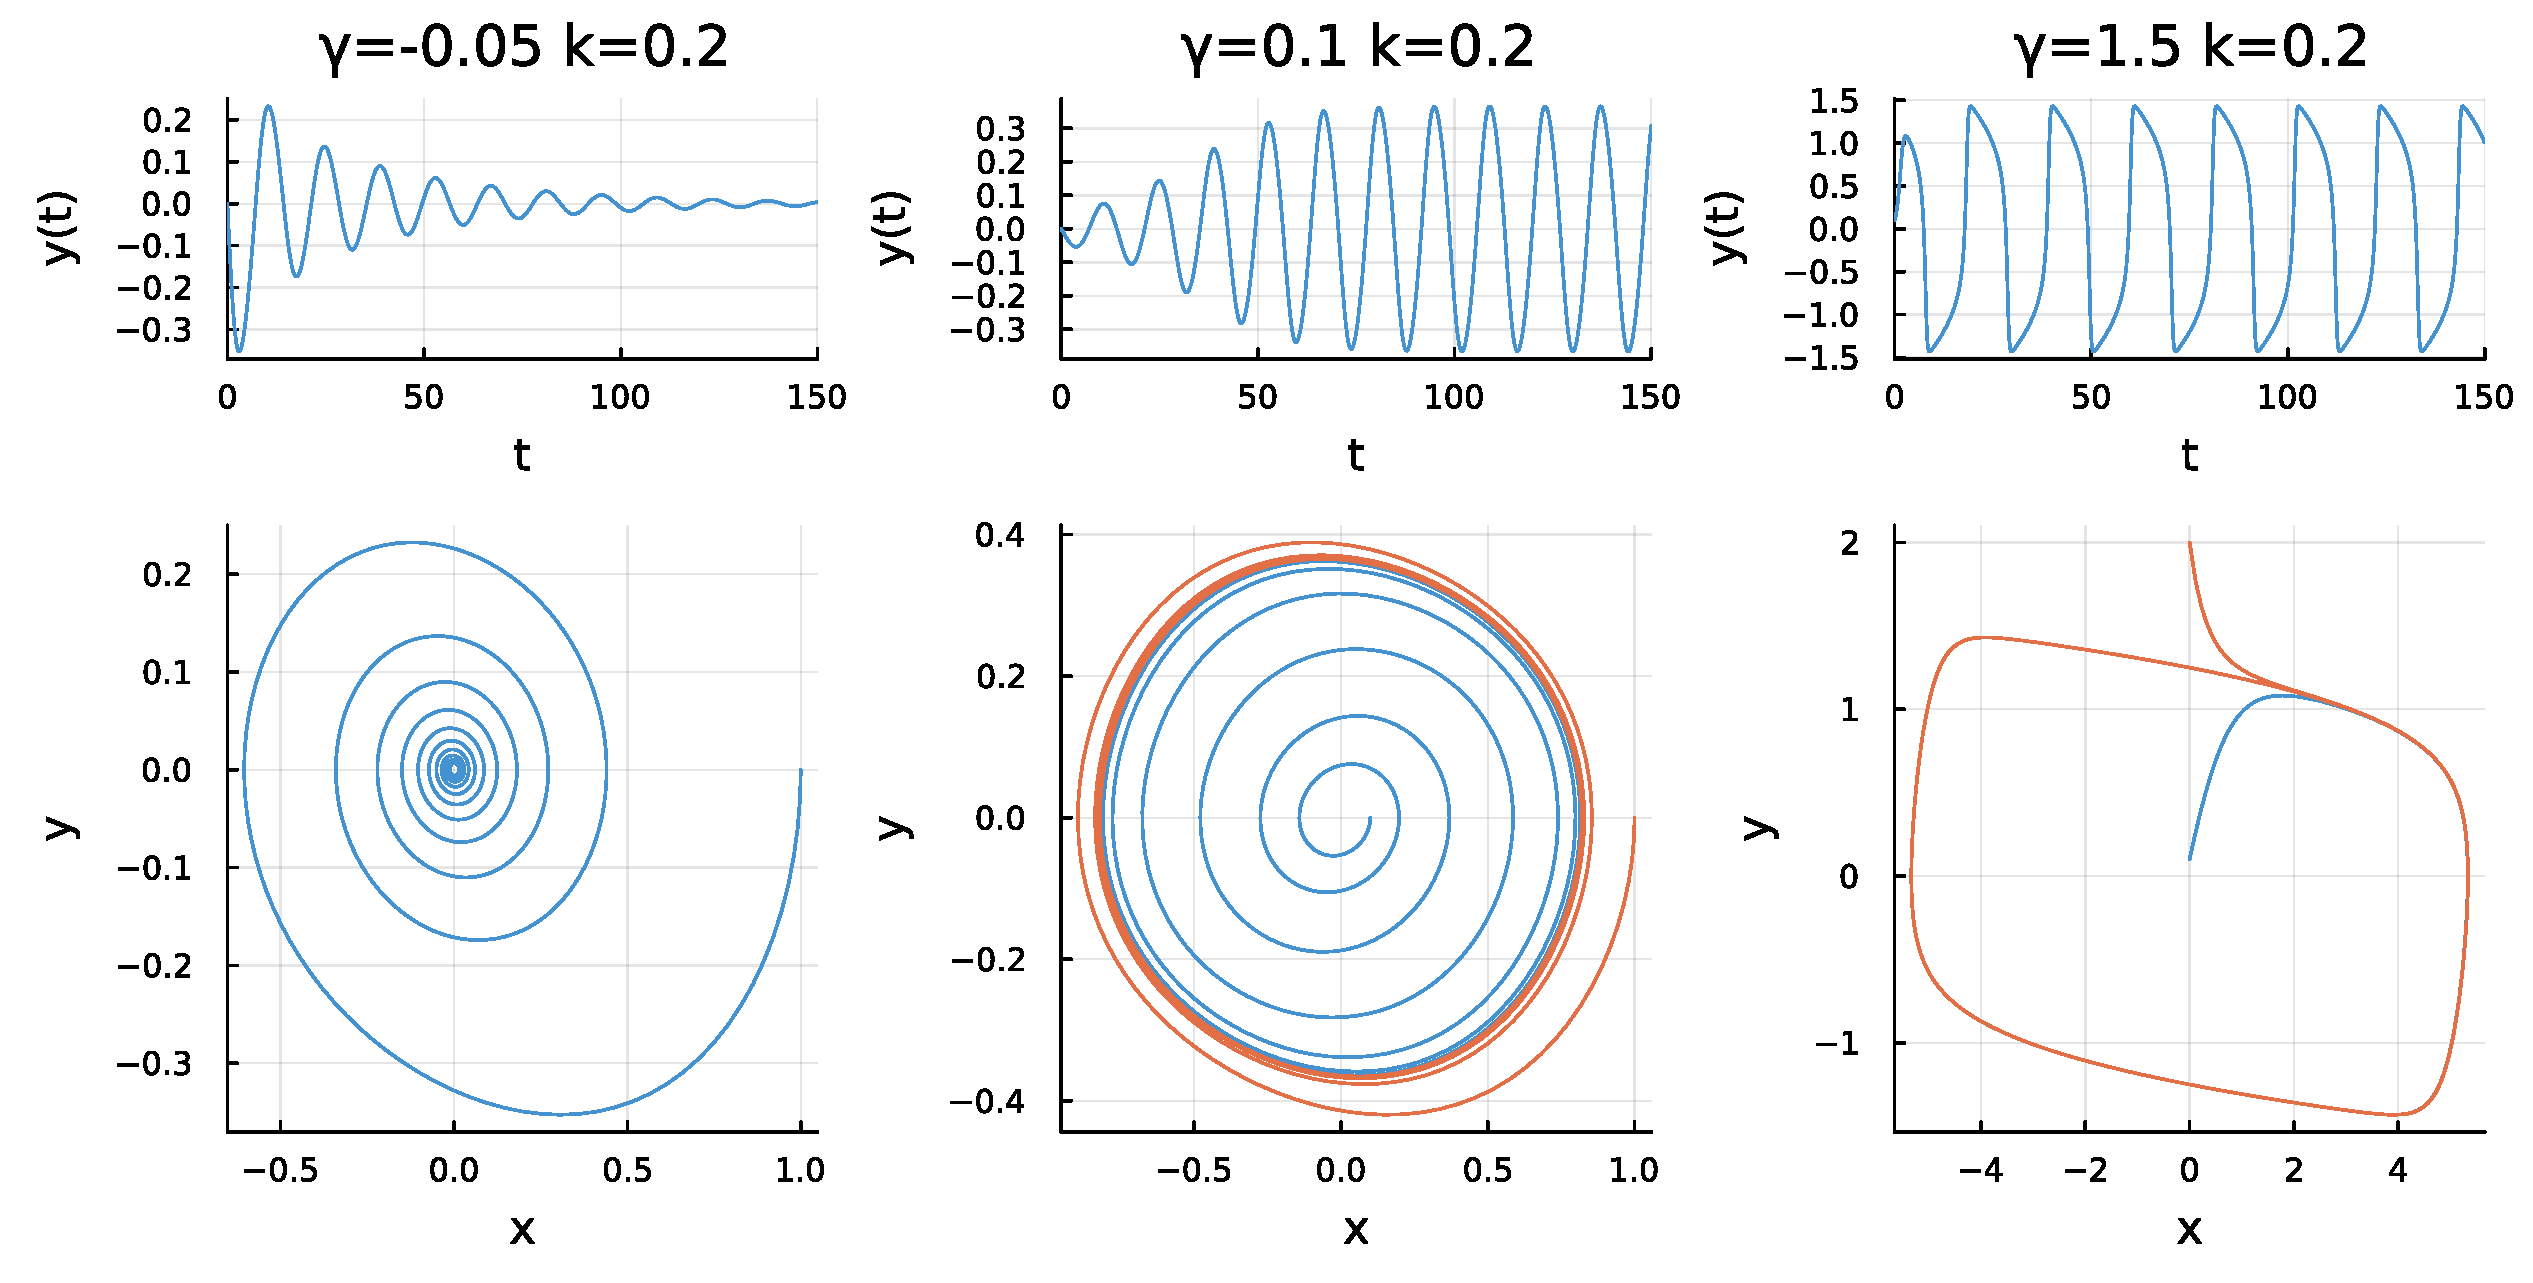
\includegraphics{figure8.eps}}
    \caption{Time evolution of the $v$ variable (top) and phase portraits (bottom) for the self-oscillator given by equation \ref{eq_selfosc} and three sets of parameters: before the Hopf bifurcation with $\gamma=-0.05$ (left), after the Hopf bifurcation with a small $\gamma=0.2$ value (center) and with a high $\gamma=1.5$ value when the relaxation oscillation is established (right).} 
    \label{fig_selfosc}
\end{figure}

The behavior of this system is displayed in Figure 8 for three values of $\gamma$ with a fixed value $k=0.2$. 
The top row shows the time evolution of $v$ for an initial condition and the bottom row shows the evolution of that trajectory in the ($x,v$) phase space.
This representation of trajectories in phase space is also known as the {\em phase portrait} of the system.
When the value of $\gamma$ is negative we have the same situation as for the harmonic oscillator with dissipation (the effect of the cubic term is to increase the resistance for higher amplitudes) and all the initial conditions evolve following spirals towards the node at the origin, as illustrated in the left column of Figure 8. 

When $\gamma$ becomes positive, the origin becomes an unstable fixed point because any small perturbation grows locally due to the positive $\gamma v$ term. 
However the system remains globally stable since for large amplitudes of oscillation the cubic term dominates and the trajectories tend towards the origin. 
These two effects combine, causing the trajectories to accumulate in an intermediate amplitude zone, giving rise to a stable limit cycle. 

This behavior is shown in the central column of Figure 8, where an outward-spiraling trajectory starting close to the origin, an inward-spiraling trajectory originating from large amplitudes, both converging to the stable limit cycle in between are represented in blue and orange lines, respectively.
 
Aditionally, when the value of $\gamma$ is positive but small the oscillations resemble those of the harmonic oscillator as shown in the center column of Figure 8 for $\gamma=0.1$. 
Note that approximately ten cycles are displayed in the time range chosen for the variable (150 time units).

As the value of $\gamma$ increases, the amplitude of the stable limit cycle becomes larger but also changes its shape, as can be seen in the right column of Figure 8. 
The periodic orbit now consists of two parts: a slow one corresponding to the slightly tilted horizontal sections and a fast one corresponding to the vertical sections of the trajectory. 
This is what is known as a {\em relaxation oscillator} and as a consequence the waveform (displayed on top) has a higher harmonic content and its frequency decreases by approximately 30 percent (seven cycles are displayed for the same time range). Also the convergence to the limit cycle is much faster.

The qualitative change that happens in this system when $\gamma$ crosses zero also constitutes a bifurcation and its type is perhaps the most common bifurcation among all natural systems that give rise to an oscillation. 
It is known as a {\em Hopf} bifurcation and is characterized by a spiral attractor point losing stability and becoming a repulsor while the system remains globally stable. As a consequence a limit cycle of low amplitude and well-defined frequency appears encircling the repulsor. This well-defined frequency for the self-oscillator described by the equations \ref{eq_selfosc} is $\omega=\sqrt{k}$.

What is the difference between the saddle node bifurcation in the circle that we saw before and the Hopf bifurcation? 
Both give rise to oscillations but with very different characteristics which are summarized in the following table.

\begin{table}[h!]
\begin{center}
\begin{tabular}{ |c|c|c| }
 \hline
 Bifurcation & Saddle-Node on Circle & Hopf \\ 
 \hline
 \hline
 Frequency & 0 &  $\sqrt{k}$ \\
 \hline
 Amplitude & finite & 0 \\ 
 \hline
 Before & Saddle and Node with an & Spiral attractor \\ 
 & heteroclinic connection & \\
 \hline
 Bifurcation & Saddle and Node collapse & Spiral loose stability \\ 
 \hline
 After & Limit Cycle & Spiral repulsor and limit cycle\\
 \hline
\end{tabular}
\caption{Saddle-Node on Circle and Hopf bifurcations compared in terms of the frequency and amplitude of the stable limit cycle created at the bifurcation point. Also a description of the dynamical scenarios before during and after the bifurcation is included.}
\end{center}
\end{table}

It is important to note that these characteristics do not depend on the specific system. 
They can even appear in systems with many variables. 
They constitute, so to speak, classes of universality in the way an oscillation can appear in the system.



\subsubsection{A self-tuned oscillator}

One drawback of the self-oscillator described by the equations \ref{eq_selfosc} is that although at the bifurcation its frequency is well defined by the parameter $k$, as the bifurcation parameter $\gamma$ increases the frequency drops dramatically. 
This can be seen in Figure 8, but also more clearly in the left panels of Figure 9. 
The upper panel displays the waveform for the $v$ variable for $k=0.2$ with two different values of $\gamma$: 0.2 (blue line) and 1.5 (orange line). 
The lower panel depicts the same for $k=1.5$. 
In both cases the waveform for the higher value of $\gamma$ is lower in frequency but this effect is much more evident for $k=0.2$.

This frequency drop appears because the trajectory of the limit cycle is gradually decomposing into two distinct sections (the diagonal and vertical sides of the relaxation oscillator) and the slow part is becoming more and more important. 
Fortunately this can be partially compensated by introducing a nonlinearity in the elastic force. 
We thus have a much more finely tuned self-oscillator given by the equations.

\begin{subequations} \label{eq_selftuned}
\begin{align}
    \dot{x} & = v \\
    \dot{v} & = \gamma y - y^3 -kx(1+0.16\sqrt{k}x^2)
\end{align}
\end{subequations}

the parameters are the same but now a new term appears with a manually adjusted value of 0.16 that partially compensates the detuning. 

\begin{figure}[h]
    \centering
    \resizebox*{17cm}{!}{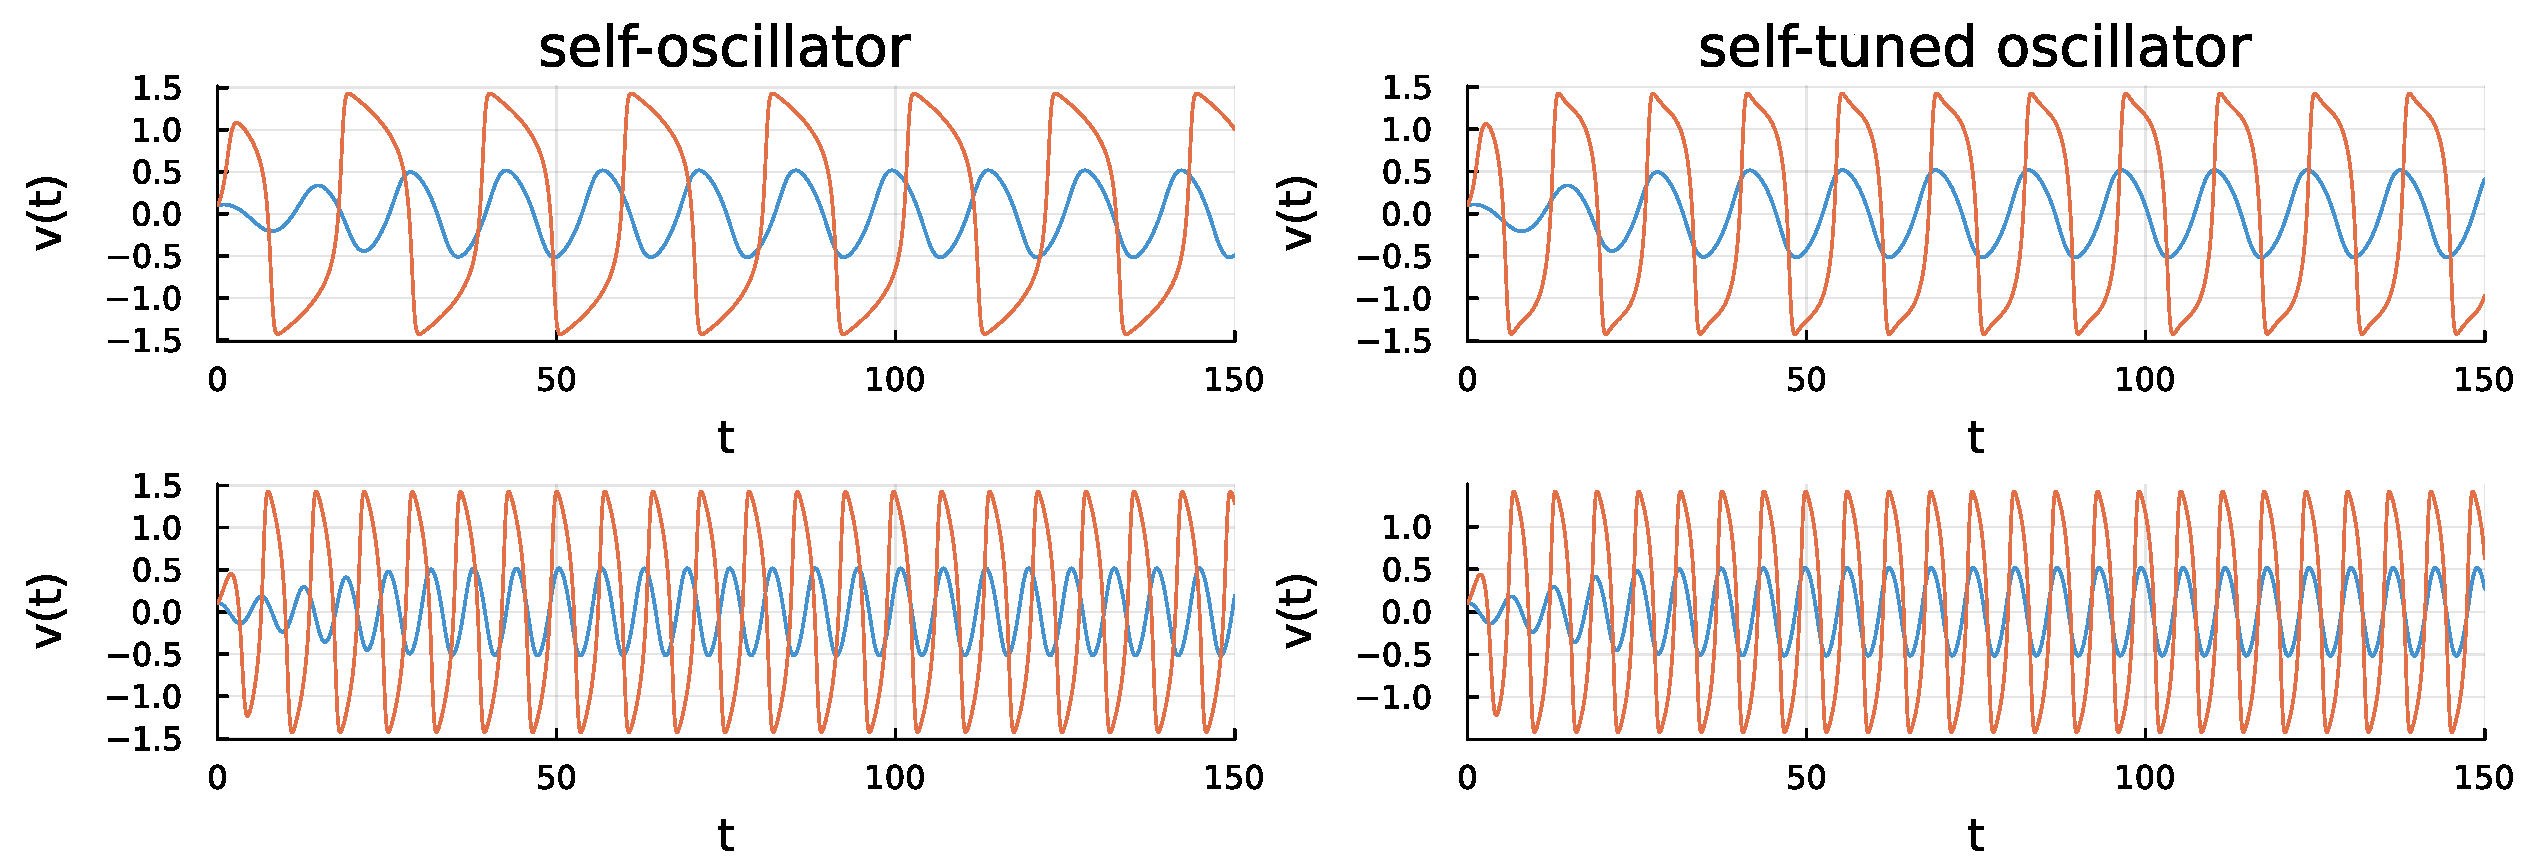
\includegraphics{figure9.eps}}
    \caption{Time evolution of the $v$ variable for the self-oscillator given by equations \ref{eq_selfosc}} (left column) and the self-tuned oscillator given by equations \ref{eq_selftuned} (right column) for values of $k=0.2$ (top row) and $k=1.0$ (bottom row) and values of $\gamma=0.2$ (blue line) and $\gamma=1.5$ (orange line). 
    \label{fig_selftunedosc}
\end{figure}

This can be seen in the right column of Figure 9 where we display the waveforms for $k=0.2$ (top) and $k=1.5$ (bottom) with two values of $\gamma$: 0.2 (blue) and 1.5 (orange), as before. 
In this case, although there is some detuning, it is clear that it is much less than in the case of the self-oscillator shown on the left.

Figure 10 shows four features of the oscillator defined by the equations \ref{eq_selftuned} plotted as a color scale in the parameter space ($k,\mu$). 
Note that unlike the phase space, each point in this space corresponds to a different system, with a different evolution and with a different phase portrait. 
In terms of sound synthesis we can think of the dynamic system as the sound generator and the parameters as external adjustment knobs that in principle serve us to explore different possibilities but that could also be modulated externally, although we will leave that for later.

\begin{figure}[h!]
    \centering
    \resizebox*{15cm}{!}{\includegraphics{figure10.eps}}
    \caption{Four characteristic mangnitudes for the self-tuned oscillator given by equations \ref{eq_selftuned} displayed as a color scale in the parameter space ($k,\gamma$): angular frequency, peak-to-peak amplitude for the $v$ variable, transient duration starting at $x=10^{-4}$, and harmonic content as a percentage} 
    \label{fig_selfcompared}
\end{figure}

The upper left panel shows the angular frequency of the oscillator, which as already anticipated depends mainly on the $k$ parameter and does not vary too much with $\mu$ (only a slight pitch bend) thanks to the additional autotuning term. 
Each thin black line separates a semitone and the thick black lines mark octaves. 
As the frequency depends on $\sqrt{k}$ here we plot $k$ from 0.125 to 2 and that corresponds to two octaves in frequency.

The upper right panel displays the peak-to-peak amplitude of the $v$ variable and it is apparent that only depends on $\mu$ (in fact it grows as $\sqrt{\mu}$). 

The duration of the transient after starting at a distances of $\epsilon = 10^{-4}$ of the fixed point is displayed in a logarithmic scale in the lower left panel. 
In this case the transient rapidly decreases after crossing the Hopf bifurcation ($\mu=0$). 

Finally, the harmonic content of the signal is estimated as the percentage increase between the mean frequency (or spectral centroid, the average frequency weighted by the spectrum amplitude) and the inverse of the period of the limit cycle (fundamental frequency) and is displayed in the lower right panel.

\subsection{Fictional frictions}

In the previous section we showed how an oscillation can be started using a negative resistance for low velocities. 
A negative resistance means a force acting in favor of the velocity, which represents a positive feedback. 
However for high speeds this resistance has to become positive, i.e. again acting against the velocity. 
We then gave the simplest form of a function that meets these requirements which involved adding a cubic term to the resistance. 

However, this is not the only way we can deliver energy to an oscillation to prevent it from dying out (which is what positive feedback represents for low velocities). 
Another possibility is that the resistance is relative to an applied external velocity. 
Imagine the mass attached to the spring but now resting on a conveyor belt with friction and moving continuously to the right as shown in Figure 11 a . 
In this case the mass will remain attached to the belt by static friction for a portion of the path. 
But static friction has a limit, as anyone who has tried to push a piece of furniture knows. 
When the elastic force pulling to the left exceeds the friction, the mass will slip and the spring will pull the mass to the left until the conveyor belt re-engages the mass and this {\em slip-stick} process repeats periodically. 

\begin{figure}[h]
    \centering
    \resizebox*{14cm}{!}{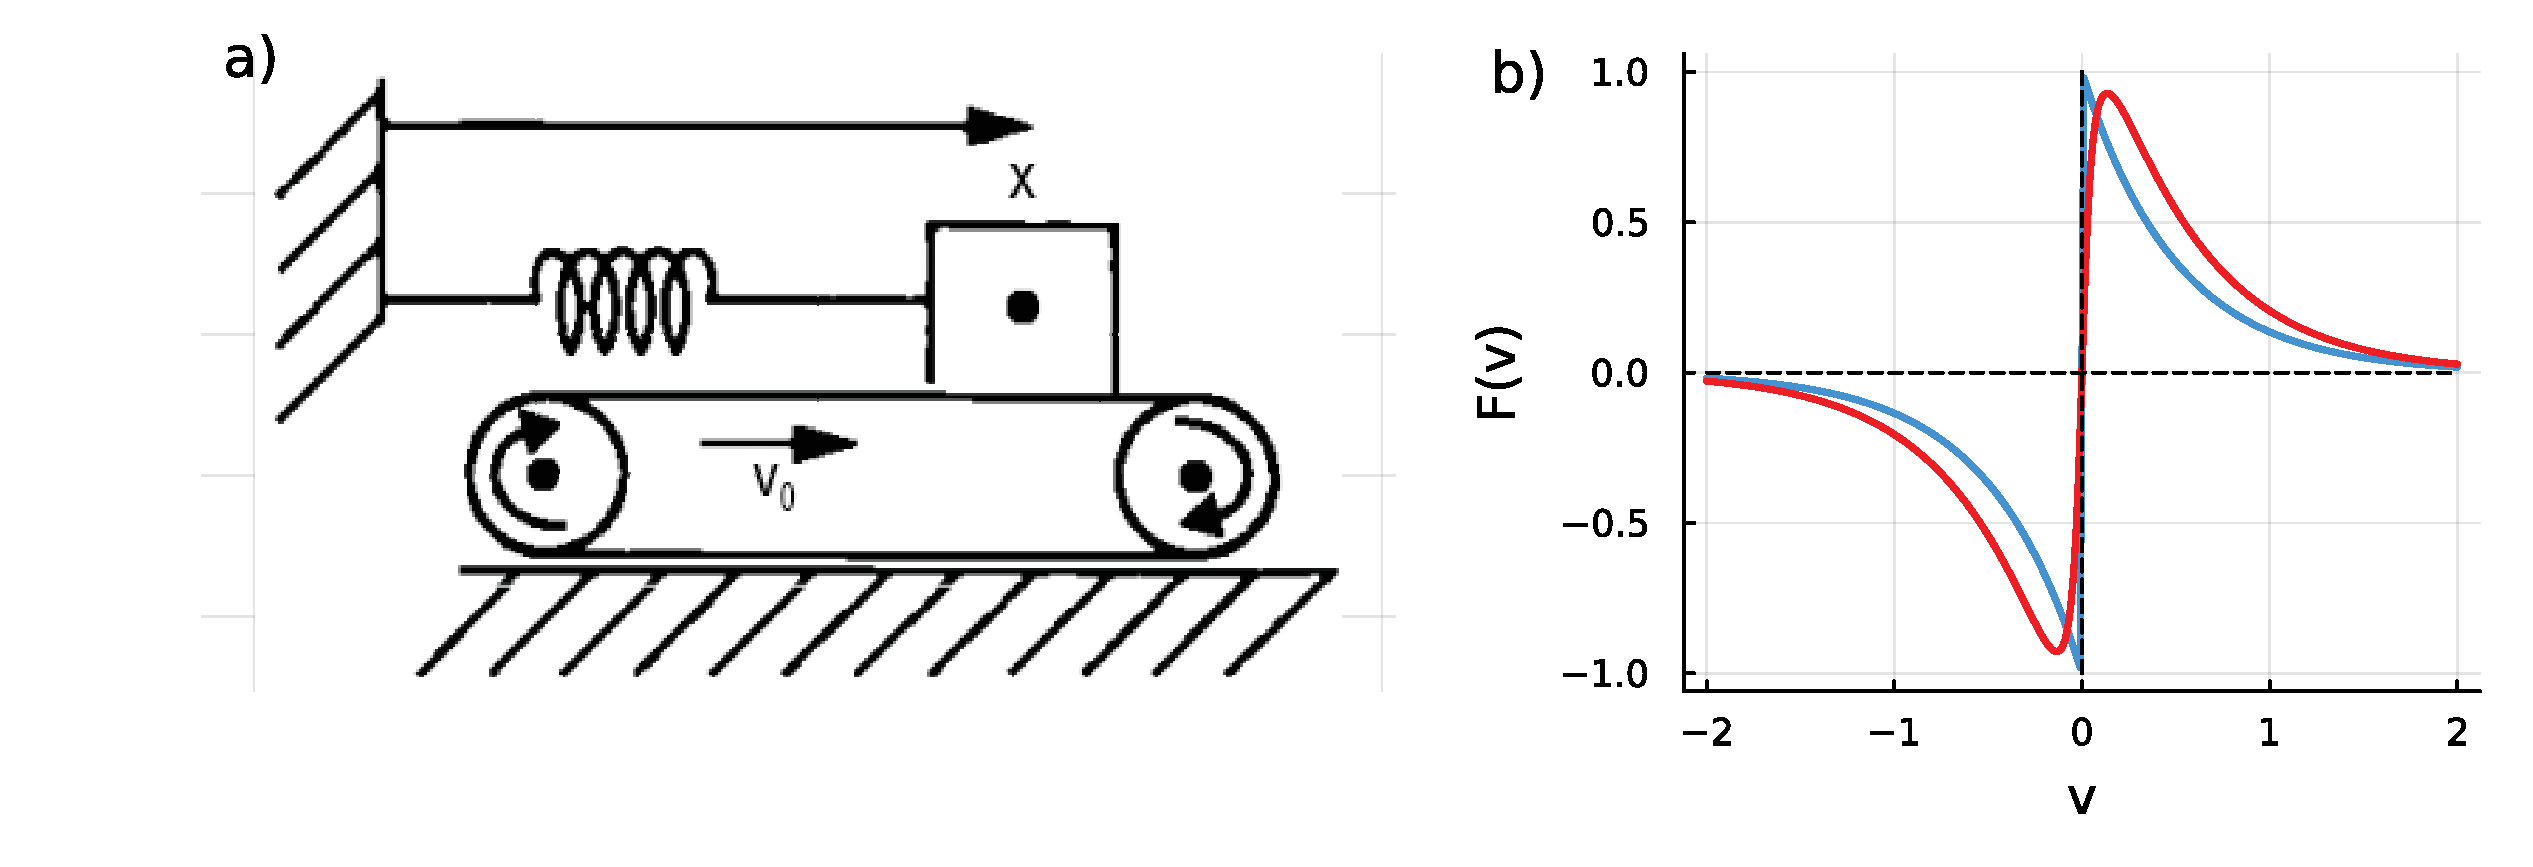
\includegraphics{figure11.eps}}
    \caption{Spring-mass system on a conveyor belt with friction: a) physical representation of the system, b) two functional forms of the friction force with (blue) and without (red) a discontinuity at the origin} 
    \label{fig_belt}
\end{figure}

This simplified system illustrates for example what happens punctually in the bow against the string of an instrument, the finger against the rim of the crystal glass or any oscillation that starts by a combination of linear displacement, surface friction and any form of elastic restitution. 
It is also responsible for the squeaking noise of shuffling chairs and many other sources of noise. 

But what are the equations describing this system like? 
In general we can write the following. 


\begin{subequations} \label{eq_bow}
\begin{align}
    \dot{x} & = v \\
    \dot{v} & = - \gamma F(v-v_0) - kx
\end{align}
\end{subequations}

where as before the term $-kx$ corresponds to the elastic restitution and $F$ is the friction acting now no longer on the velocity of the mass but on the difference of the velocity of the mass with the conveyor belt of velocity $v_0$. 
Now we must imagine how is the form of this force. 
One requirement for $F$ is that it must be very high for very low velocities and decrease as the velocity increases. 
Of course, it must also always oppose the motion. 
Notice that as we now put the negative sign outside the function it must be positive when $v>v_0$ (the mass is sliding on the belt pulled by the spring) and negative when $v<v_0$ (something that can happen on the left if the spring pushes the mass at a higher velocity than the belt). 
It is also reasonable to assume that this force is symmetric in both directions. 
Thus, we need a function that is positive on the right that starts at a high value and begins to decay and on the left that is the same but from the negative. 

A simple possibility is shown in Figure 11.b in blue $F(v) = \text{sgn}(x) e^{-2|v|}$. 
However we are going to use a “smoothed” version of this function (to avoid the discontinuous jump to zero) which is shown in the red curve in Figure 11.b and has the functional form:

\begin{equation} \label{eq_bowfriction}
    F_{bow}(v) = \arctan(v/\epsilon) e^{-2|v|} 
\end{equation}

where $\epsilon$ is a small regularization parameter (we use $\epsilon = 0.05$).
The behavior of the system defined by equations \ref{eq_bow} with the friction force given by equation \ref{eq_bowfriction} is displayed in Figure 12 for three parameter values. 
For the sake of simplicity we will fix $k=1$ in the following.

For small values of $|v_0|$ the slope of $F$ is positive, resulting in a single stable fixed point, as shown in the left column of Figure 12.
Every initial condition evolves spiraling down towards that fixed point. 
The function $F(v-v_0)$ as a function of $v$ is also depicted by the 
orange line. Therefore the fixed point is always located at the intersection of this curve with the horizontal line $v=0$.

\begin{figure}[h]
    \centering
    \resizebox*{15cm}{!}{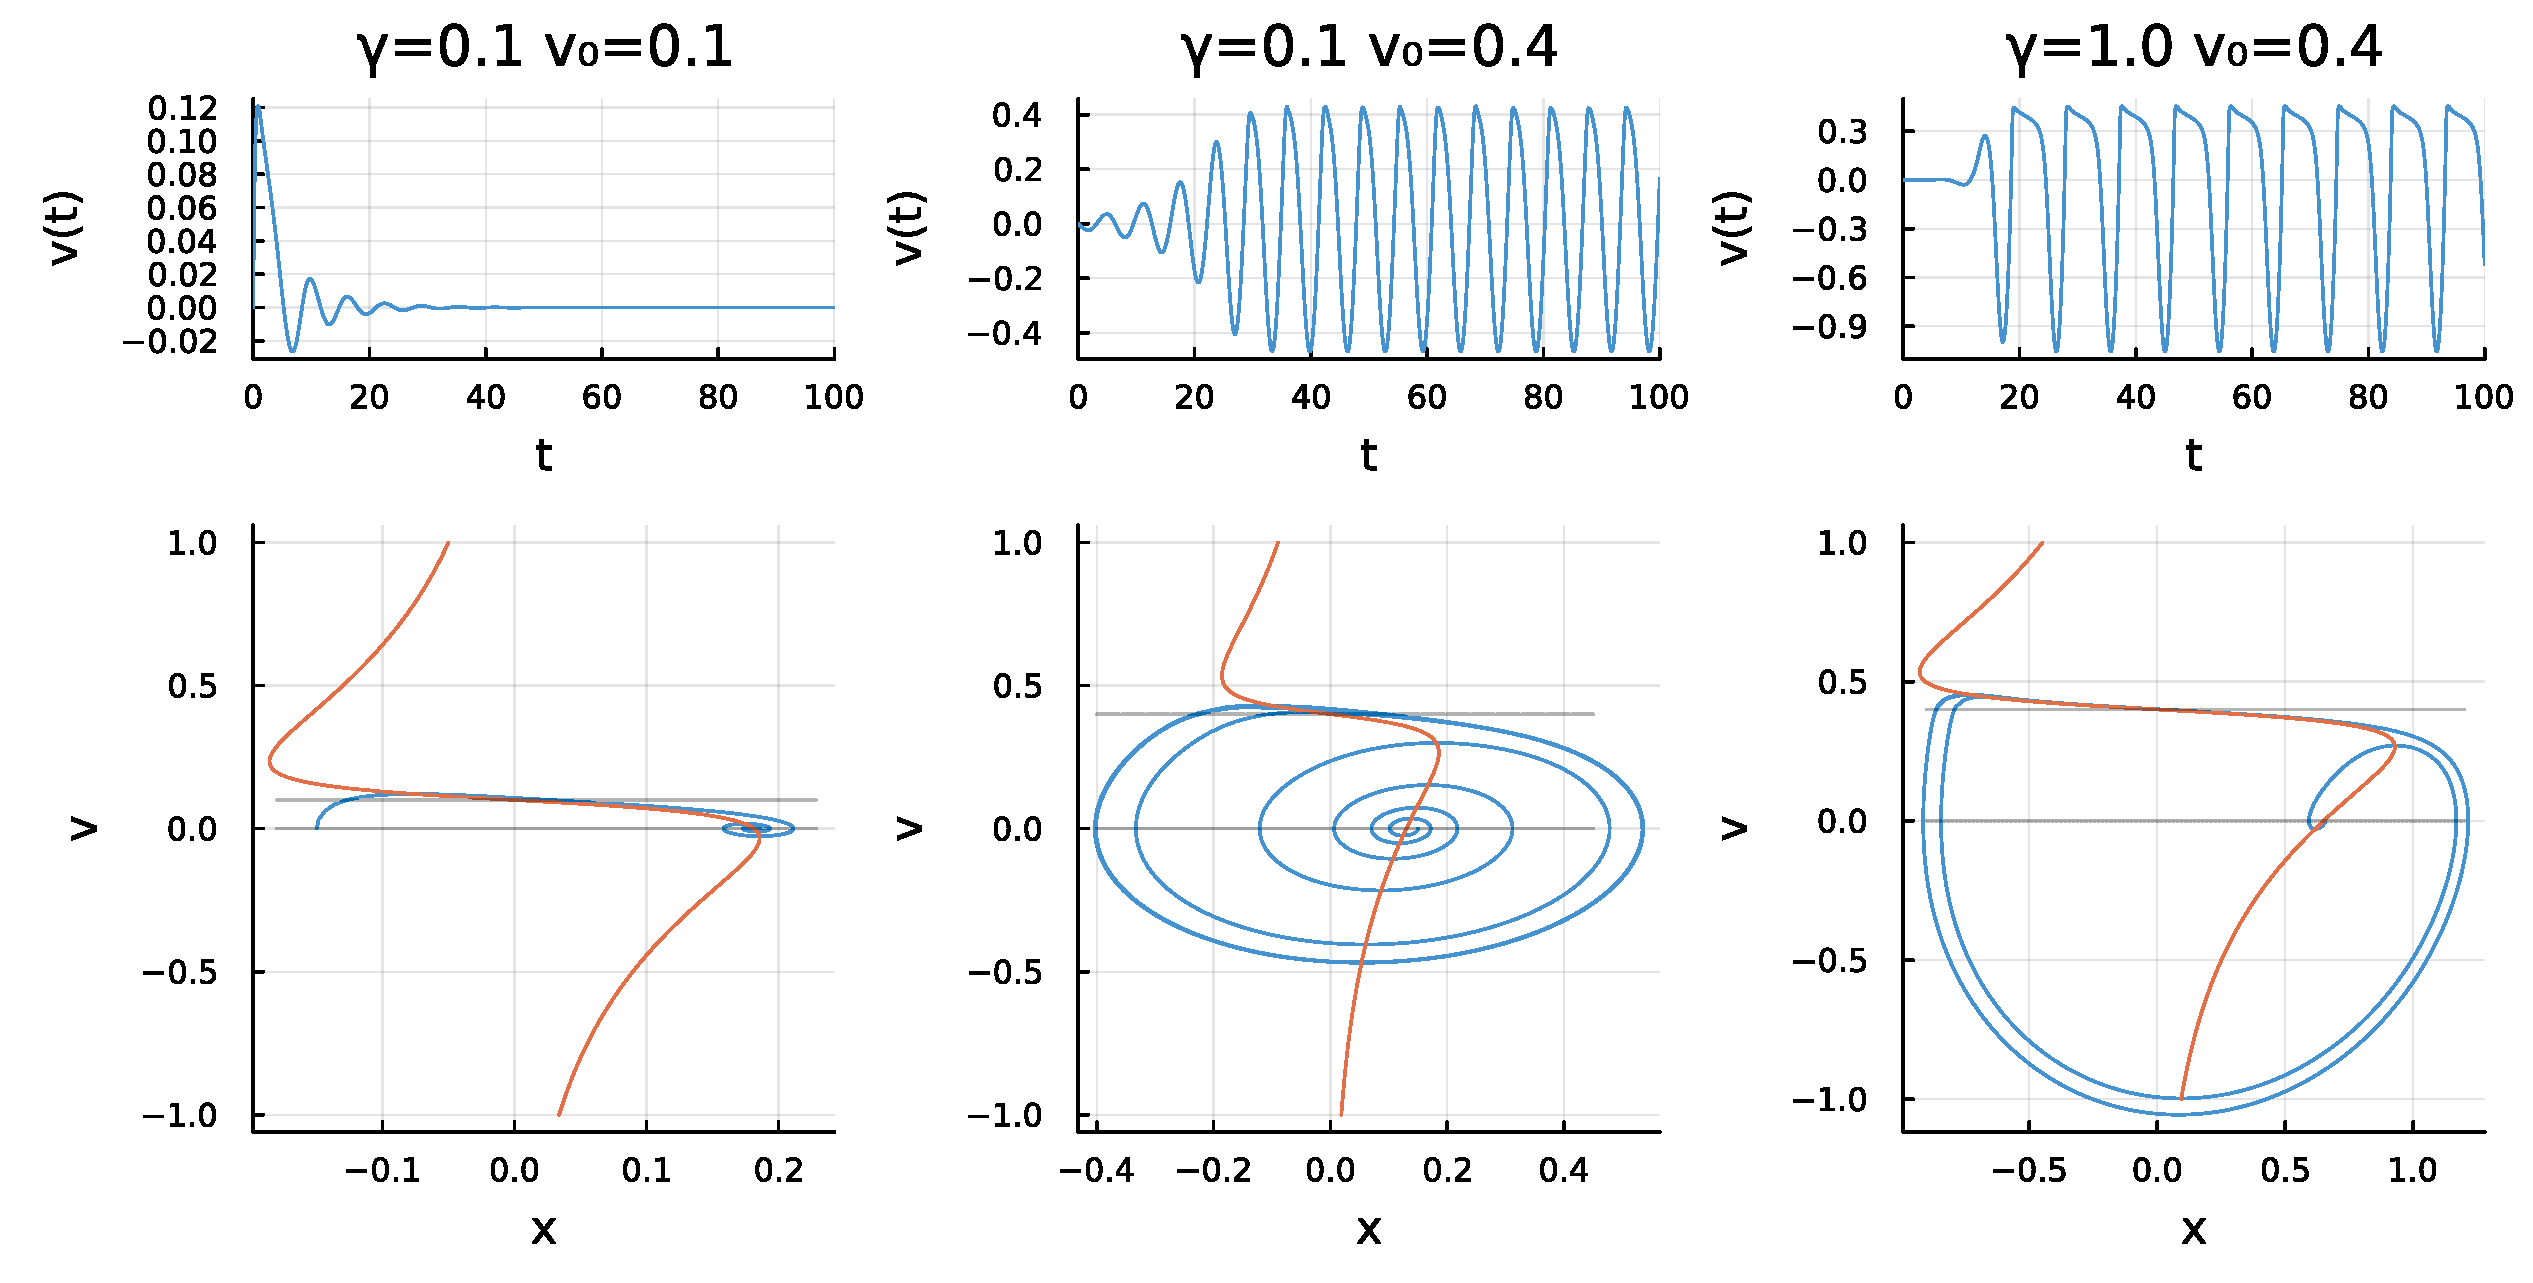
\includegraphics{figure12.eps}}
    \caption{Time evolution of the $v$ variable (top) and phase portraits (bottom) for the system given by equations \ref{eq_bow} with the functional form for the friction of equation \ref{eq_bowfriction} that models the physical system of Figure 11. The left column displays the system before the Hopf bifurcation with only a stable fixed point and the center and left columns display the system after the Hopf bifurcation with a stable limit cycle for two values of the friction parameter $\gamma$} 
    \label{fig_bow}
\end{figure}

As $v_0$ increases, the fixed point shifts to a region of the  $F$ curve where the slope is negative. In this region, the fixed point loses stability, undergoing a Hopf bifurcation that gives rise to a stable limit cycle with a small amplitude. 
This behavior is illustrated in the central column of Figure 12.

Note that the shape of the limit cycle is flattened at the top and that in that part it follows closely the curve of $F$. 
This portion of the cycle corresponds to the moment when the mass is dragged by the conveyor belt and does not slip so the velocity difference with the belt is minimal. 
When it reaches the right side the trajectory takes off downwards returning with a negative velocity (slipping) towards a point on the left where it reattaches to the belt. 
This behavior is much more evident on the right column of Figure 12 where the friction is higher therefore the mass is stuck much stronger to the belt while being dragged. 
The waveform obtained has the timbral characteristic of rubbed instruments or slip stick processes in general with a series of triangular pulses followed by flat sections.

Finally it is worth noticing that the same behavior can be observed with a negative $v_0$ but in this case the mass slips in the other direction and the limite cycle is reversed in both coordinates.

\subsubsection{Other frictions (Saddle-Node of Limit Cycles)}

As a last example we will explore other "fictional" forms of friction, in the sense that they do not necessarily have to replicate a physical system (although for some of them it might be possible to find examples). 
In particular we are interested in a system in which the oscillations are created (or destroyed) by a mechanism different from the two seen so far (Saddle-Node on the circle or Hopf). 
The system is given by the equations with the following functional form for the friction:

\begin{equation} \label{eq_fictional}
    F_{fictional}(v;\sigma) = v - v^3 + \sigma v^5  
\end{equation}

The parameter $\sigma$ accompanying the fifth order term will be responsible for the bifurcation that will give rise to (or end) the oscillations.
This functional form alternates positive and negative sections and results in the creation of an unstable limit cycle in addition to the stable one. 
This unstable limit cycle will form a {\em separatrix} that will divide the phase space into two {\em basins of attraction}: an inner one where all initial condions will converge to a stable fixed point and an outer one where all the initial conditions will converge to the stable limit cycle. 

To understand how this is reflected in the behavior of the system we can examine the phase portrait displayed in the first two columns of Figure 13. 
An initial condition inside the unstable limit cycle is shown there in blue that spirals inward toward the center where there is a stable fixed point. 
An initial condition at a point with a slightly larger value of the coordinate (on the other side of the unstable limit cycle) displayed in orange spirals outward until it is trapped in a neighbourhood of the stable limit cycle. 
The difference is that when the parameter $\sigma$ is small the separatrix is close to the origin and almost all initial conditions end up in the unstable limit cycle, which has the form of a large relaxation oscillator and square waveform. 
As $\sigma$ increases the unstable limit cycle grows in size and the stable one shrinks so that they end up very tightly spaced, as can be seen in the middle column of Figure 13. 
For a value of $\sigma$ between 0.22 and 0.23 both cycles collapse in what is known as a Saddle-Node bifurcation of limit cycles and only the stable fixed point remains at the origin as can be seen in the right column of Figure 13. 

Of course, if we traverse this bifurcation backwards (decreasing the value of $\sigma$) we have that a stable limit cycle (together with an unstable one) is created “out of nothing” in a region of phase space. 
Therefore this is a qualitatively different form in which an oscillation can appear and is characterized by the occurrence of oscillations of finite amplitude (as in the Saddle-Node on the circle) but with definite frequency (as in the Hopf).




\begin{figure}[h]
    \centering
    \resizebox*{15cm}{!}{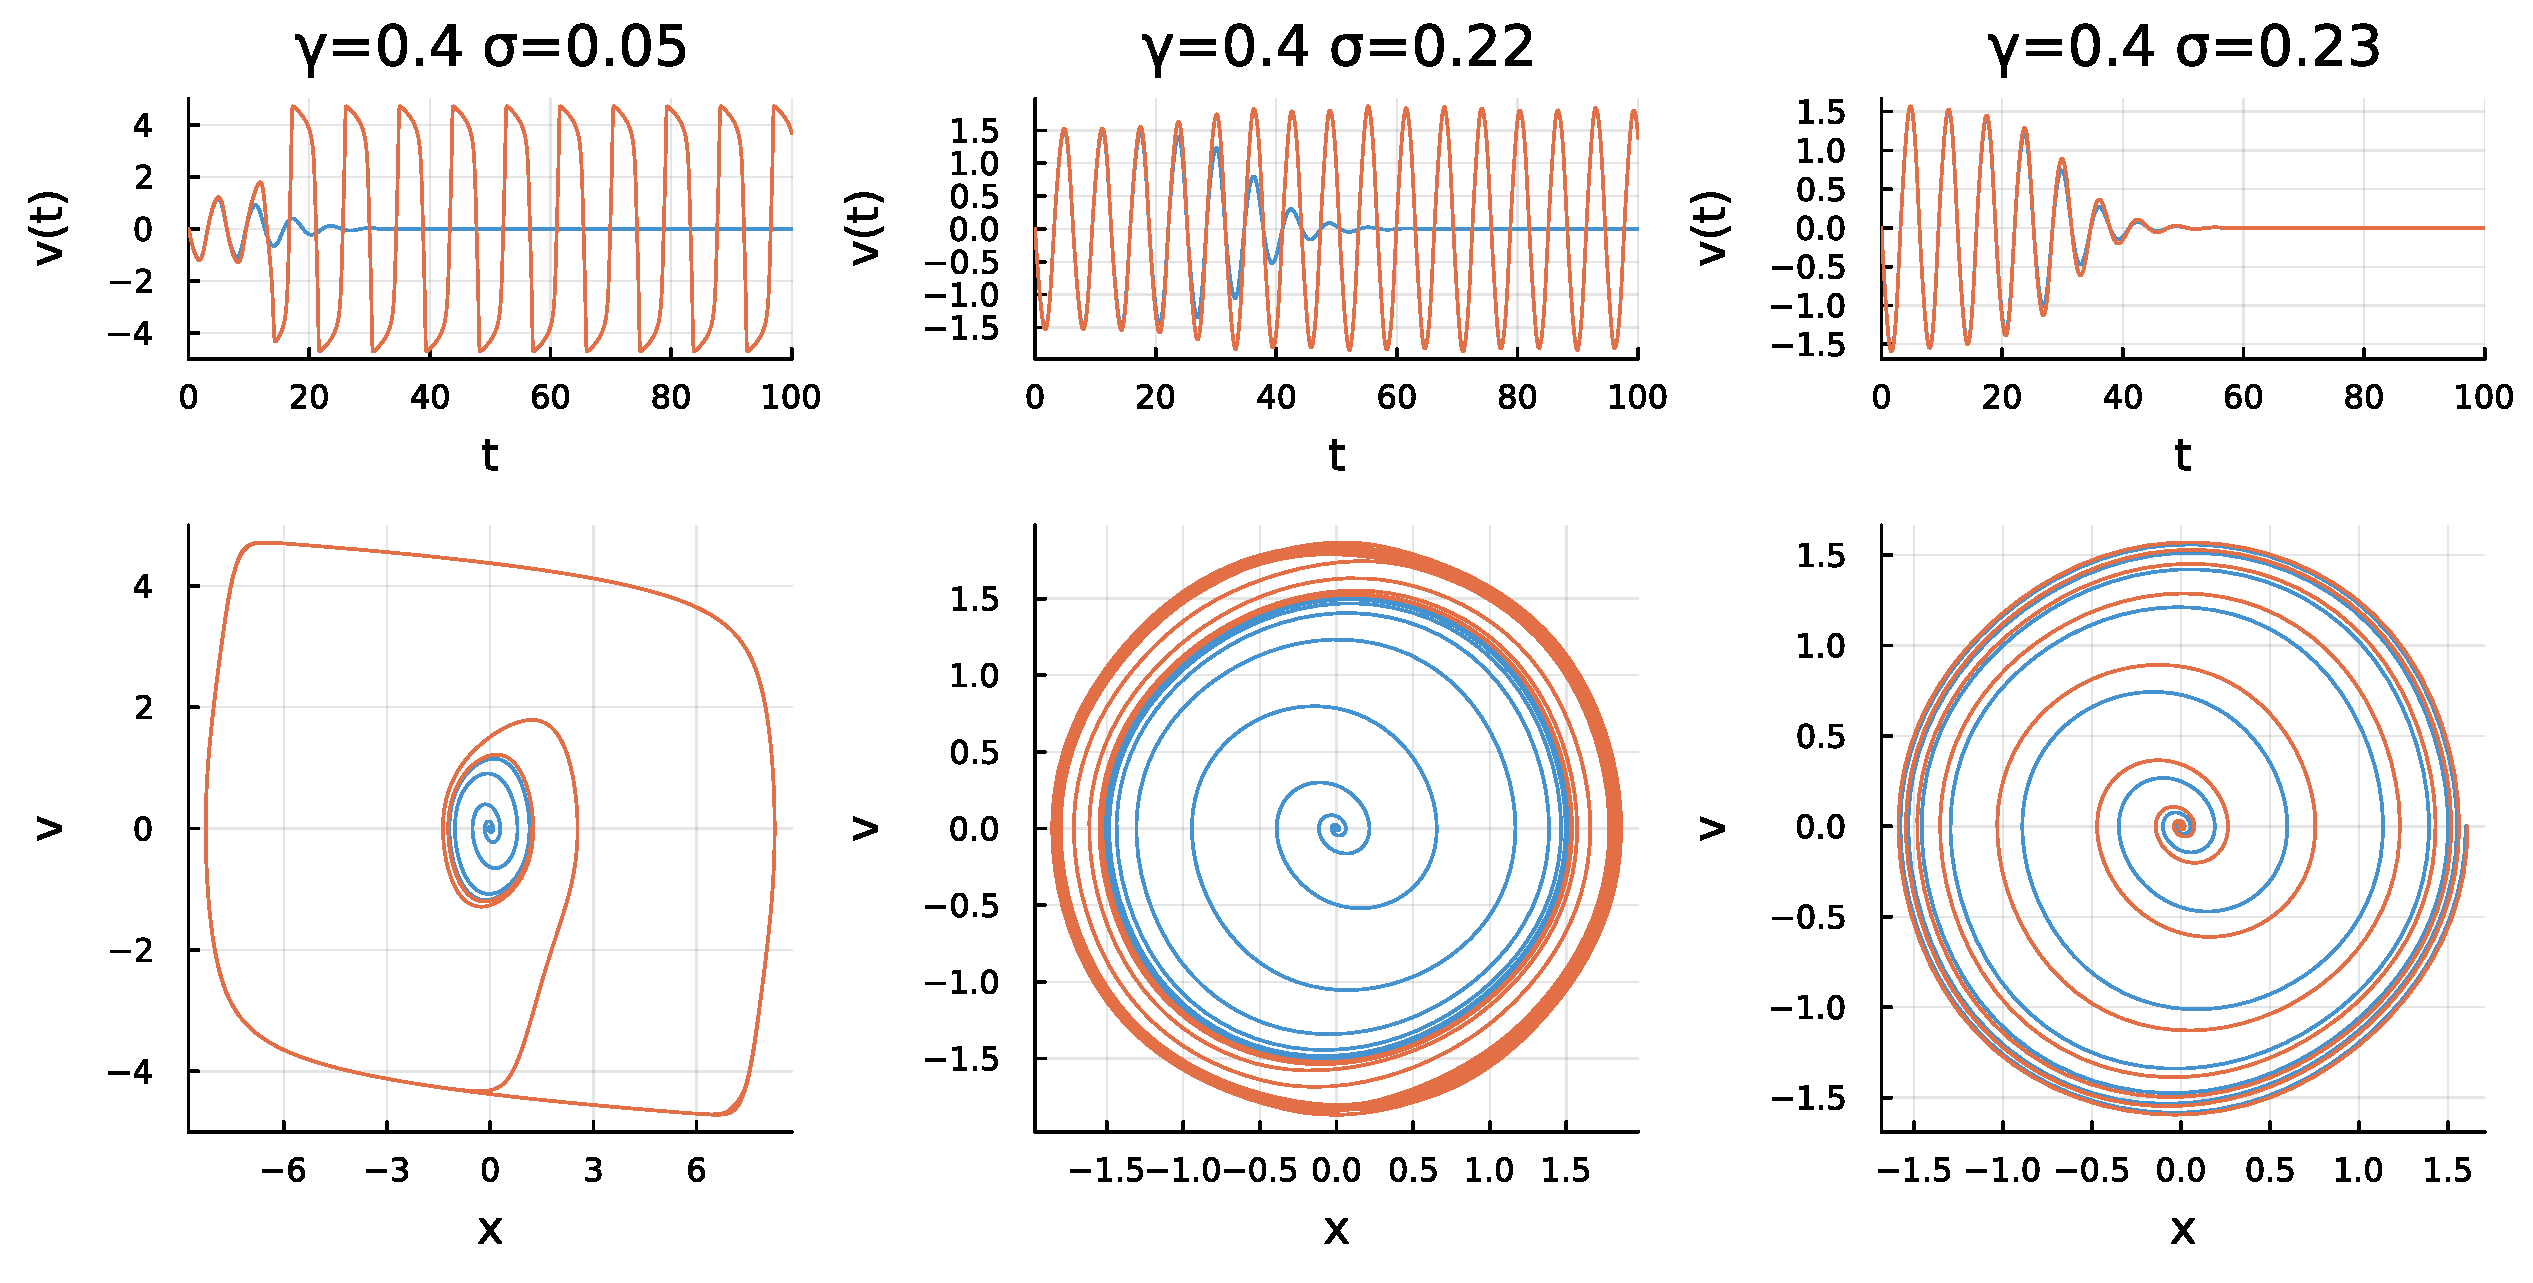
\includegraphics{figure13.eps}}
    \caption{Time evolution of the $v$ variable (top) and phase portraits (bottom) for the system given by equations \ref{eq_bow} with the functional form for the friction of equation \ref{eq_fictional} for three $\sigma$ values. On the two first columns an unstable limit cycle divides the phase space in an inner region with trajectories decaying to a stable fixed point in the center (in blue) and an outer region with trajectories converging to a stable limit cycle (orange). In the left column the stable limit cycle has a clear relaxation oscillator form. In the right column both limit cycles collapsed in a Saddle-Node of Limit Cycles bifurcation and all trajectories decay towards the origin.} 
    \label{fig_friction2}
    
\end{figure}

\subsection{The meaning of a saddle (Homoclinic Bifurcation)}

There is an additional, qualitatively different, mechanism by which a limit cycle (and hence an oscillation) can be created/annihilated at least in two-dimensional phase space and it corresponds to a homoclinic bifurcation. 
This bifurcation involves a saddle point which so far did not intervene so much in the scenario except in the bifurcation on the circle and it had not been clear why we called it a saddle and not merely a repulsor. 

So before showing the bifurcation let's see how the flow behaves in an neighborhood of different types of fixed points and that will allow us to understand the meaning of a Saddle.

\begin{figure}[h]
    \centering
    \resizebox*{17cm}{!}{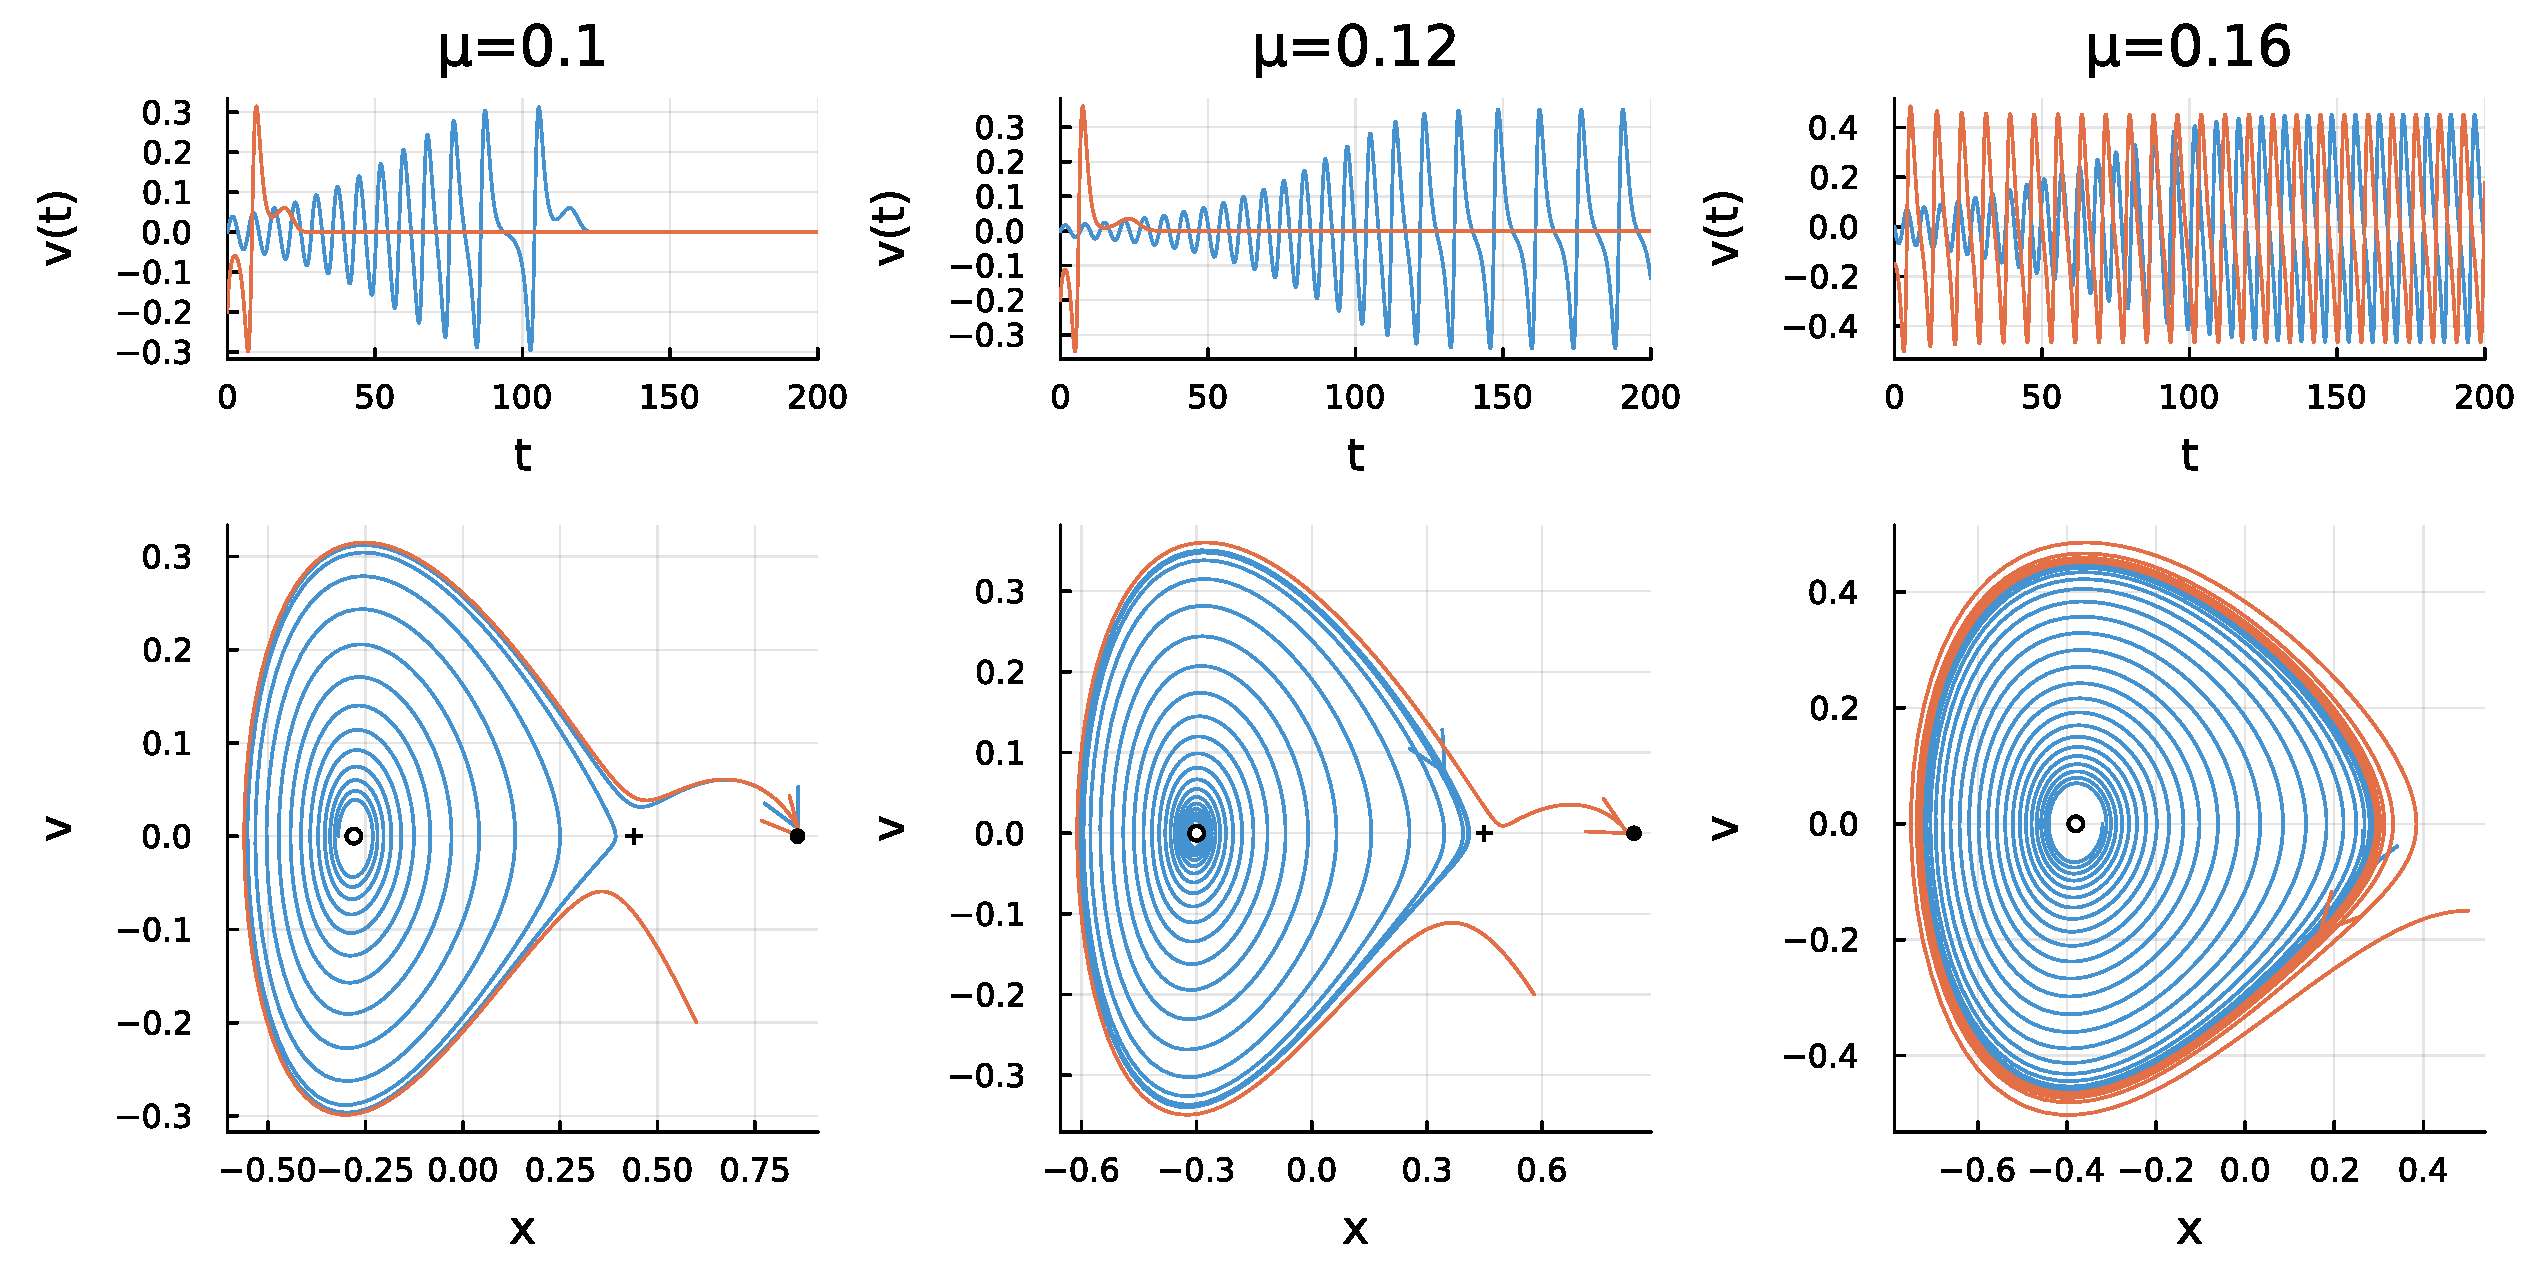
\includegraphics{figure14.eps}}
    \caption{Five classes of fixed points in the plane, from left to right: (SA) spiral attractor, (NA) node attractor, (S) saddle point, (NR) node repulsor, and (SR) spiral repulsor} 
    \label{fig_homoclinic}
\end{figure}

Figure 14 shows a qualitative diagram of the flow around five categories of fixed points in the plane. 
The first two on the left are stable or attractors and they differ in that the flow goes directly to them following straight lines as in the attractor node (NA) or forming a spiral as in the attractor spiral (SA). 
The latter was the fixed point that changed stability in the Hopf. 
The two on the right correspond to unstable fixed or repulsor points, either repulsor nodes (NR) or spirals (SR). 
The fixed point in the middle is the Saddle and as can be seen it has two different directions. 
In one direction it is an attractor and in the other a repulsor, therefore the flow approaches it in a grazing way. 
Note also that, with the exception of the two straight trajectories that end in the fixed point all the others circulate approaching the Saddle without touching it. The portion of the trajectory that is close to the Saddle also is slowed down dramatically.
A very relevant feature of saddle points is that they act as watersheds or flow separatrices, often separating different basins of attraction. As can be seen, the stable direction acts in this way and the trajectories that are to its left or right are sent to different destinations in the unstable direction.

\begin{figure}[h]
    \centering
    \resizebox*{17cm}{!}{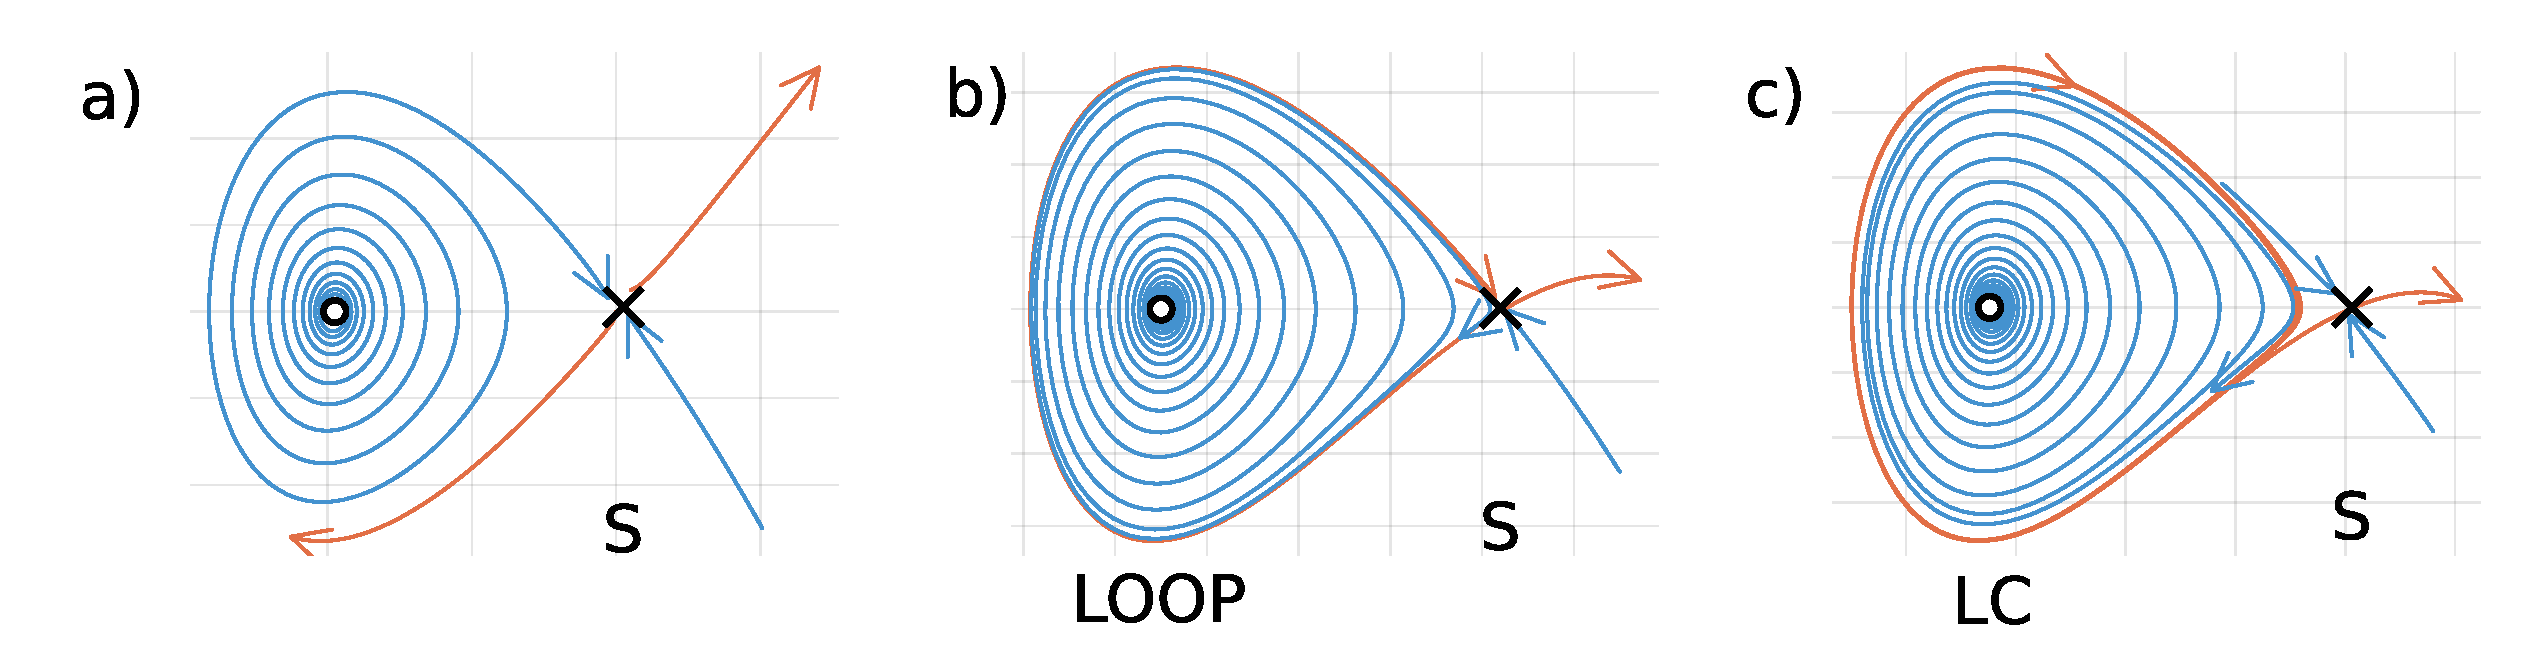
\includegraphics{figure15.eps}}
    \caption{Homoclinic bifurcation: a) a Saddle point (S) is feeded by an spiral repulsor (white circle); b) at the bifurcation point it forms a saddle loop; c) after the bifurcation a stable limit cicle (LC) is emitted from the loop} 
    \label{fig_homoclinic}
\end{figure}

The homoclinic bifurcation involves the encounter of a saddle with a stable limit cycle. 
And the consequence of that encounter is the anhilation of the limit cycle. 
If we imagine that one of these trajectories approaching the saddle is a stable limit cycle we will have a slowing of the flow and the behavior of the oscillation would be as shown in Figure 15.c. 
By modifying the system parameters in the homoclinic bifurcation the limit cycle collides with the Saddle forming a loop (or homoclinic connection) as shown in figure 15 b. 
That loop can be seen as the limit cycle slowing down to such a length that it is now an infinite period orbit. After the bifurcation the limit cycle disappears (Figure 15.a).
If we traverse the bifurcation from left to right in Figure 15 we can see how a stable limit cycle is created when a saddle point forms a homoclinic connection or loop. And then after the bifurcation that loop detaches from the saddle forming a stable limit cycle. This is a new mechanism by which an oscillation can be turned on.

Let's see an example of a system that generates oscillations by this bifurcation. The system is given by the following equations:

\begin{subequations} \label{eq_homoclinic}
\begin{align}
    \dot{x} & = v \\
    \dot{v} & = \delta xv + x^2 - x^3 -x^2v - \mu
\end{align}
\end{subequations}

For this case we fix $\delta=0.5$ and explore $\mu$ that will be our bifurcation parameter. 

\begin{figure}[h!]
    \centering
    \resizebox*{15cm}{!}{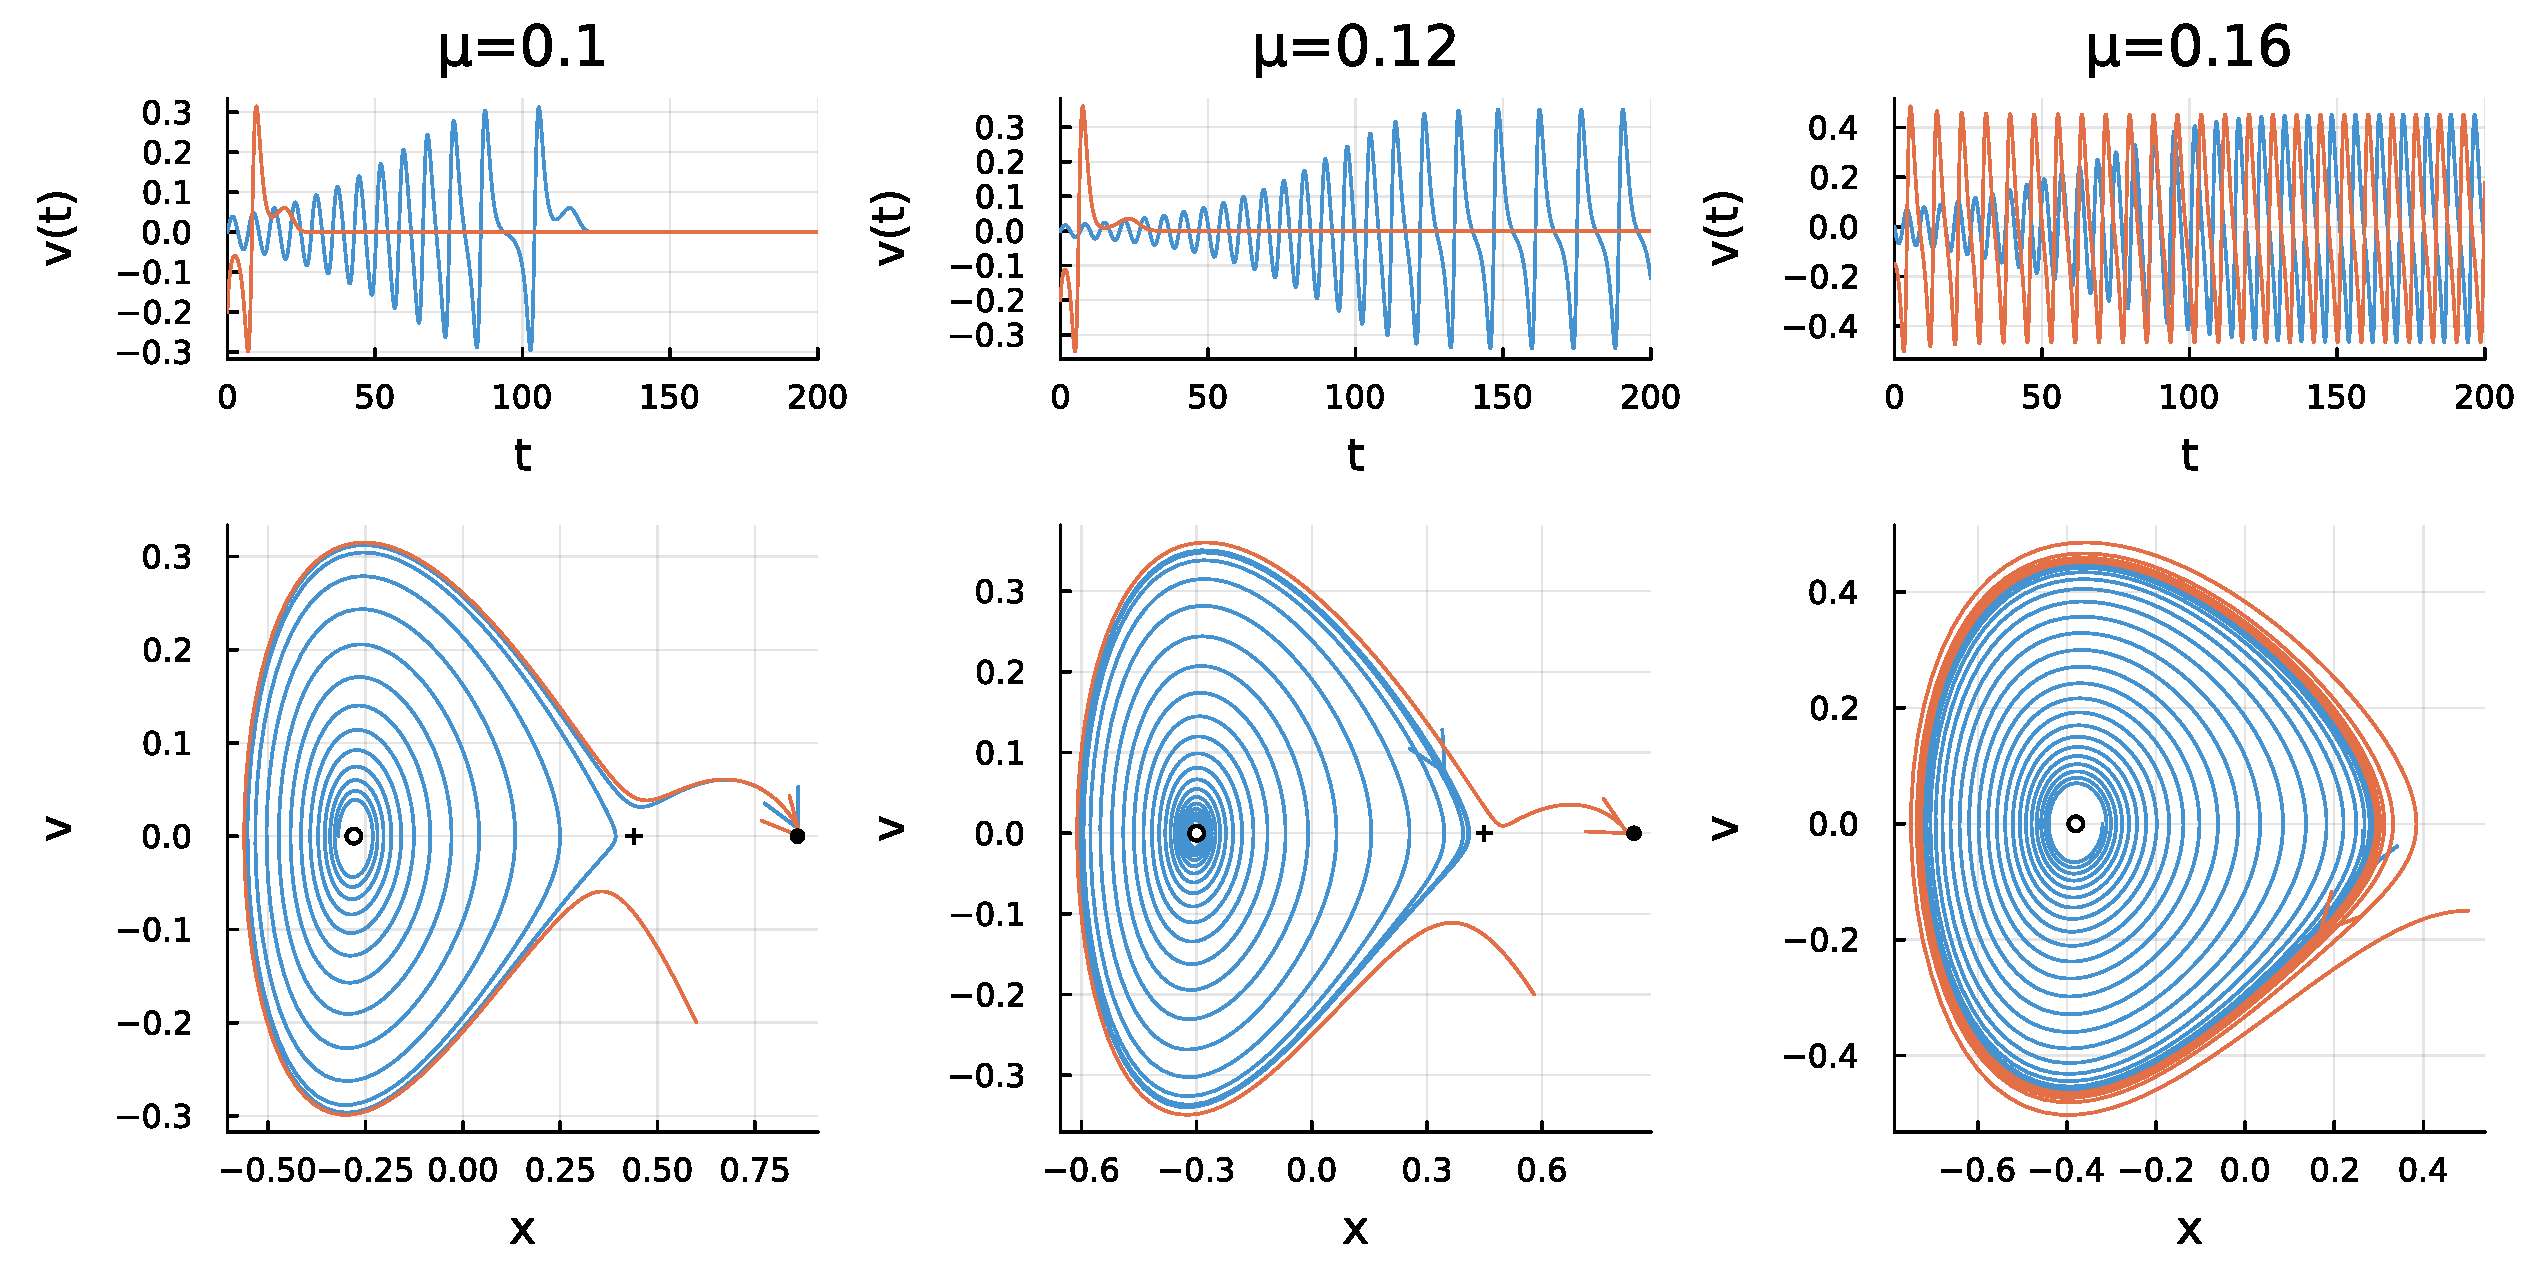
\includegraphics{figure16.eps}}
    \caption{Time evolution of the $v$ variable (top) and phase portraits (bottom) for the system given by equations \ref{eq_homoclinic}.
    unstable fixed point (white circle), saddle point (cross), stable fixed point or node (black circle). An homoclinic bifurcation occurs around $\mu=0.11$. Before the difurcation (left) all trajectories end at the sstable fixed point. After the bifurcation the system is bi-stable some trajectories end at the stable fixed point and others at the newly created limit cycle (cente). Finally after a Saddle-Node bifurcation all trajectories end up in the stable limit cycle.} 
    \label{fig_homoclinic}
\end{figure}

In Figure 16 we display as before the time evolution of the $v$ variable on top and the phase portraits on the bottom for three $\mu$ values. 
On the first two phase portraits there are three fixed points indicated by symbols: an unstable spiral (white circle), a saddle point (cross) and a stable node (black square). 
In the first column, all initial condition end in the stable node, so there. is no oscillation. 
However there are trajectories, like the blue one, that approach the saddle almost touching it. 
One of these trajectories will form the homoclinic connection at the bifurcation. 




In the central column the scenario after the bifurcation ($\mu=0.12$) is displayed: a stable limit cycle is formed and all initial conditions inside it end up on the cycle (blue line). 
Also, a very thin region outside converges into it, 
However, other trajectories are deflected by the saddle separatrix and end at the attractor node (orange line). 
In this regime the system behaves as bi-stable because it has two possible competing behaviors: an oscillatory one shown by the blue trajectory and a stationary one shown by the orange trajectory.

Finally, in this system there is one more bifurcation but that does not affect the limit cycle. 
In the right column it can be seen that for $\mu=0.16$ the saddle and the node disappeared (in an ordinary Saddle-Node bifurcation) and therefore only the limit cycle remains. 
The system is no longer bi-stable and the behavior is purely oscillatory for all initial conditions.

To conclude this part we can summarize in a table the behavior of the four bifurcations that can turn on an oscillation by completing the previous table:

\begin{table}[h!]
\begin{center}
\begin{tabular}{ |c|c|c|c|c| }
 \hline
 Bifurcation & SN on Circle & Hopf & SN of Limit Cycles & Homoclinic\\ 
 \hline
 \hline
 Frequency & 0 &  $\sqrt{k}$ & arbitrary & 0\\
 \hline
 Amplitude & finite & 0 & finite & finite \\ 
 \hline
 Before & Saddle and Node with an & Spiral attractor & & Saddle\\ 
 & heteroclinic connection & & &\\
 \hline
 Bifurcation & Saddle and Node collapse & Spiral loose stability & Limit Cycle Neutral & Homoclinic connection\\ 
 \hline
 After & Limit Cycle & Spiral Repulsor & Pair of Stable/Unstable & Saddle and Stable\\
 & & Limit Cycle & Limit Cycles & Limit Cycle\\
 \hline
\end{tabular}
\caption{The four bifurcations compared}
\end{center}
\end{table}

\subsection{Questionnaire}
\begin{enumerate}
\item Draw a qualitative phase portrait for the harmonic oscillator with no damping $\gamma=0$ for different initial conditions.
\item Why the "simplest" form of the negative resistance is $\gamma v - v^3$? Why there are no quadratic terms?
\item Explore the limit of high damping (high $\gamma$ values) and low frequency (low $k$ values) for the self-oscillator. What happens with the relaxation oscillator?
\item Imagine a MIDI controlled musical instrument using the self-tuned oscillator. Propose a mapping between the parameters ($\gamma,k$) and the key note and velocity. 
\item How does the parameter $k$ influence the frequency of the resulting sound in the simplified bow model given by the equations \ref{eq_bow} and \ref{eq_bowfriction}? 
\item And in the above model for a fixed $k$, how does the parameter $v_0$ influence the sound frequency?
\item Explore the same dependence in the fictional frequency model given by the equations \ref{eq_bow} and \ref{eq_fictional}. When the stable and unstable limit cycles arise, do they do so with a given frequency?
\item What happens if we add a perturbation in the $x$ variable near the homoclinic bifurcation in the model given by equations \ref{eq_homoclinic}?
\end{enumerate}

\end{document}

\section{One dimensional oscillations in systems with delay}

\subsection{The "simplest" system}
\begin{equation}
    \dot{x} =  x(t-\tau)-x(t-\tau)^3 - \gamma x 
    \label{eq_delay}
\end{equation}

\begin{figure}[h]
    \centering
    \resizebox*{17cm}{!}{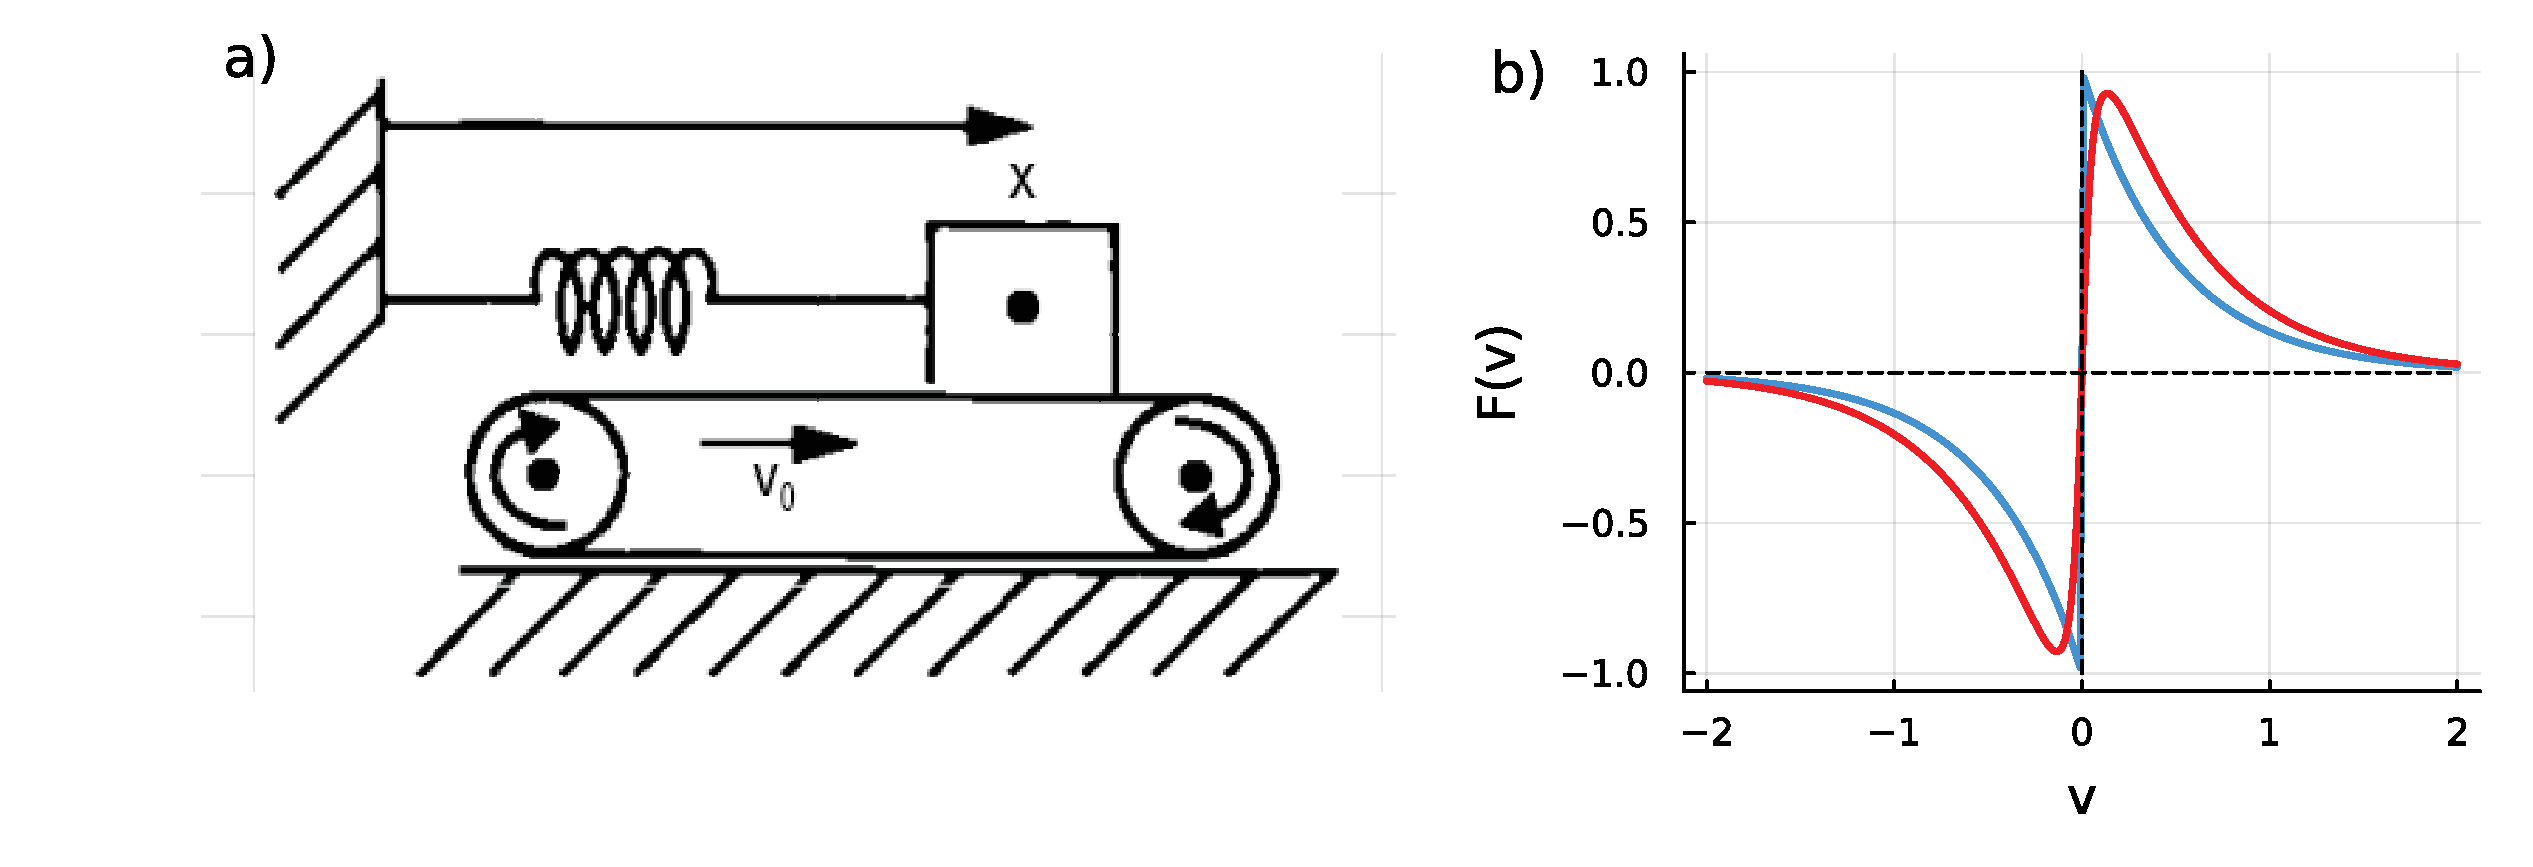
\includegraphics{figure11.eps}}
    \caption{} 
    \label{fig_delay}
\end{figure}


